
\chapter{AARSim: An Integrated High-fidelity Simulation Platform for Autonomous Aerial Refueling}

Aerial refueling has been extensively researched over the last decade and received conspicuous achievements because of its advantages of increasing the endurance and range of aircraft. A complete aerial refueling process includes a variety of interdisciplinary platform modeling (aircraft aerodynamic modeling, flexible hose modeling, complex wind interference, airflow interference between aircraft, etc.) and various complex perception and control tasks (robust visual recognition and tracking, reliable flight control, formation, and coordination control, high-precision air docking control). Existing platforms focus on some aspects of aerial refueling due to the lack of a complete set of high-fidelity simulation, test, and development platforms suitable for the entire process of aerial refueling. Therefore, this paper proposes an integrated high-fidelity simulation platform for autonomous aerial refueling. The platform includes high-precision motion models (including receiver model, tanker model, and hose-drogue model), a high-fidelity 3D simulation that supports visual sensors' output, multi-functional control interface (unmanned autonomous controller, manual joystick control), multiple complex disturbance models and injection interfaces such as wind disturbance and the mass change of receiver. Hence the platform can simulate the dynamics and kinematics of motion models, support selection, setting, and output of different sensors, and demonstrate the entire aerial refueling process in a high-fidelity 3D simulation. Furthermore, algorithms test and development can also be implemented in this platform. In the verification part, two demos implemented in the platform show that the proposed platform can accomplish the entire aerial refueling mission by designing the guidance, navigation, and control algorithms with autonomous and manual methods. The source code of this platform is released, making it easier to study the related work of aerial refueling. 

\section{Introduction}
\label{sec1}

Autonomous aerial refueling (AAR) has become increasingly popular because of the rapid development and use of unmanned aerial vehicles (UAV)\cite{thomas2014advances,nalepka2005automated,quan2014survey}    which attract the attention of many scholars in colleges and institutions. Significant progress has been made over the last decade. Autonomous refueling programs were drawn up by the US at the beginning of this century and were mainly implemented by three agencies, NASA, USAF, and US Navy. NASA's Autonomous Airborne Refueling Demonstration (AARD) project has been declared successful with the X-47B completing its first mid-air refueling in April 2015. US Navy completed the mid-air refueling test\cite{Nottdmct} with F/A-18F in the summer of 2021. In March 2023, Airbus Defense and Space announced that it had conducted an autonomous aerial refueling test with a multi-role tanker transport (MRTT) that can control the UAV without human intervention\cite{aaiag}. 

However, it is almost impossible for researchers in colleges or other institutions to conduct aerial refueling flight tests, which puts forward requirements to build integrated high-fidelity simulation platforms. This motivates some institutes to build aerial refueling simulation platforms. Aerospace Vehicles Technology Assessment and Simulation(AVTAS) laboratory established a human-in-the-loop refueling scenario using simulation consoles for a boom operator, tanker pilot, and UAV operator, which is built on the commercially available simulation platform D-Six and can run one tanker and four UAV aerodynamics models\cite{burns2005automated}. This AAR real-time simulation platform with a high-fidelity boom operator station is comparatively complicated and only supports flying boom refueling. In Ref\cite{pollini2003virtual}, a virtual platform for UAVs' aerial refueling using the probe-and-drogue method is established based on MATLAB$ ^{\rm{TM}} $/Simulink$^\circledR$ and commercial software DynaWORLDS. However, the platform is mainly used to test vision-based algorithms. German Aerospace Center gave a general overview of the performed modeling work, some specifics in selected parts of the model, and the developed simulation infrastructure for the aerial refueling scenario. However, the proposed AVES full-flight research simulator is challenging to build for other researchers\cite{FEZANS2018116}. 

To facilitate the comprehensive modeling, simulation, test, and development of AAR, this paper establishes a high-fidelity simulation platform for aerial refueling based on MATLAB$ ^{\rm{TM}} $/Simulink$^{\circledR}$, named AARSim. As shown in Figure \ref{FIG_1}, current aerial refueling systems can be divided into three types: flying-boom type, probe-and-drogue type, and boom-drogue-adapter type. AARSim adopts the probe-and-drogue type because the modeling, disturbances, and control of this type are more complicated. What's more, this type can be applied in multi-aircraft refueling, which is helpful for swarm combat. Users can re-develop other types of platforms based on AARSim. 

\begin{figure}[th]
	\centering
	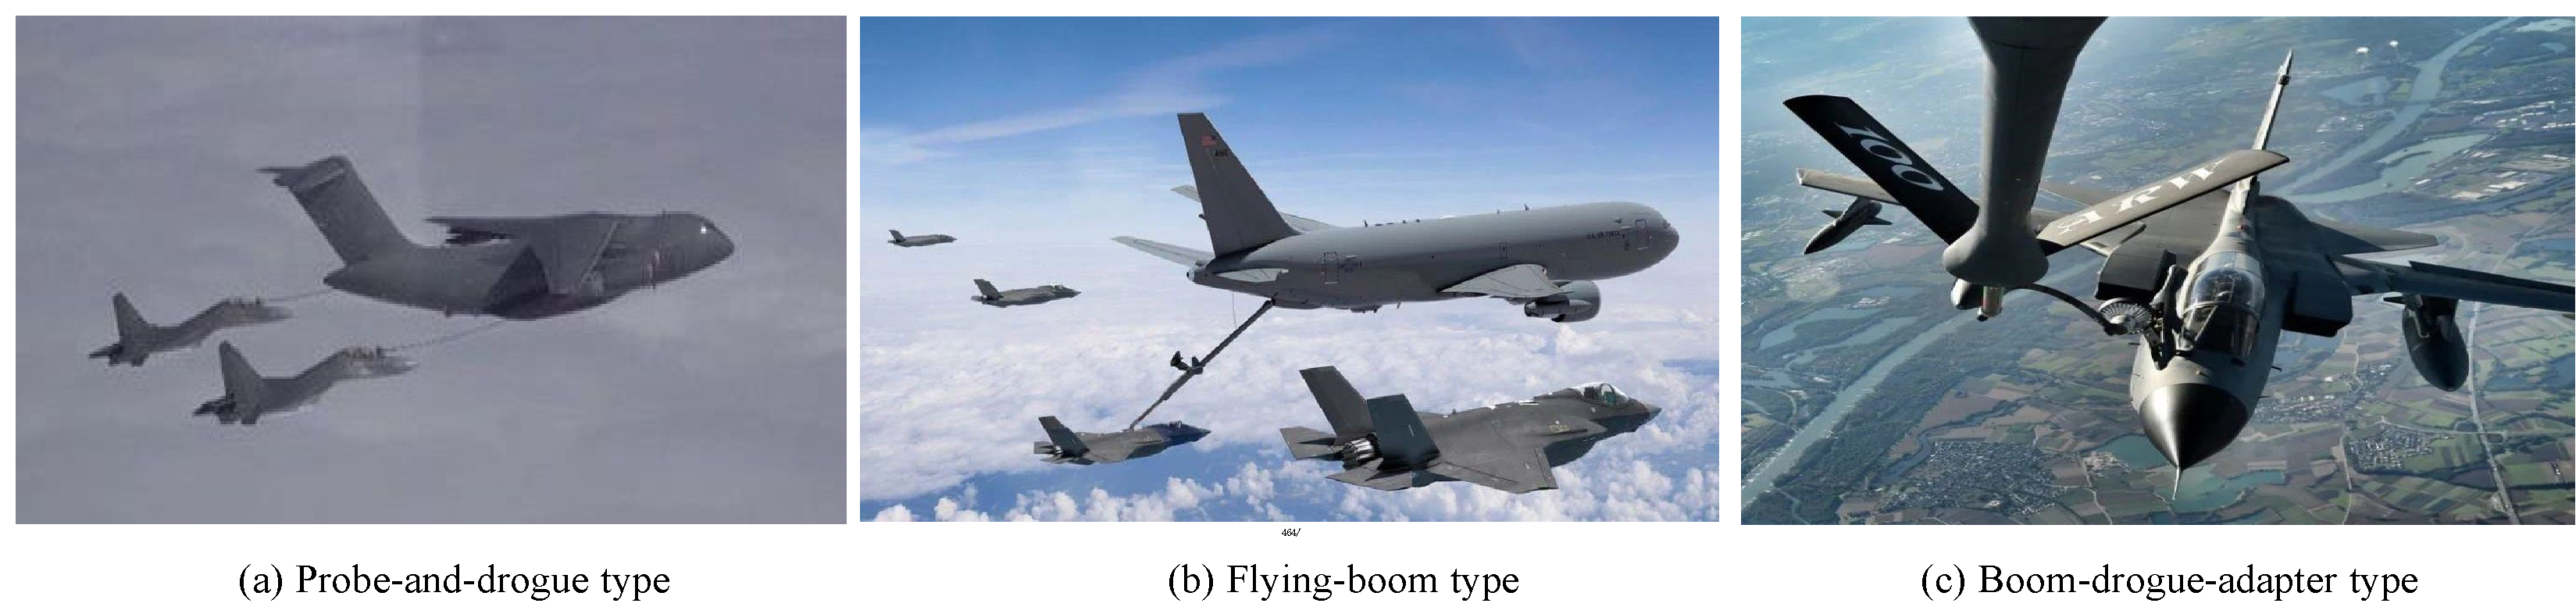
\includegraphics[width=1\textwidth]{Figures/Figs_Ch5/Fig1.pdf}
	\caption{Three types of aerial refueling systems.}\label{FIG_1}
\end{figure}

The modeling of AARSim is as follows. In a typical AAR process, a tanker enters a racetrack orbit to wait for rendezvousing with receivers, which requires that the tanker not perform a high maneuver. As a result, it is generally assumed that the tanker maintains steady-state flight. A hose with a drogue at its end is attached to a hose-drum-unit (HDU) in the tanker, which is modeled by the finite element method\cite{wei2016drogue}. The HDU is a reel take-up system abling to effectively suppress the hose whip (HWP)\cite{ro2011dynamics,wang2014dynamic,dai2019hose,wang2015dynamics}. The tanker can generate wake turbulence trailing from its lifting surfaces. The modeling includes the vortex lattice model, the roll-up vortex model, and so on. Besides wake turbulence, the Dryden\cite{moorhouse1980us} model usually represents atmospheric turbulence and the ``1-cosin" Gust model for wind gusts. The bow wave effect is modeled with explicit equations to simulate the real flight conditions\cite{wei2016drogue,dai2016modeling}. The aircraft models (including tanker and receiver) usually take the form of 6-DoF rigid body dynamics. Refueling can change the receiver's state more than that of the tanker because tankers are often bigger. As a result, a mass-varying receiver model is adopted\cite{ma2018formation}. Particularly, the 3D visualization model supports the real-time dynamic status display of the aircraft and the hose-drogue model, perception of visual\cite{arafat2023vision} information obtained by sensors\cite{parry2023review}. The control in AAR mainly refers to the receiver. For the receiver, there are three distinct control tasks through the refueling process: (1) trajectory generation for rendezvousing, (2) station keeping with the tanker, and (3) docking the drogue. Various control methods can be employed, such as the feedback method, the linear quadratic regulator(LQR), terminal iterative learning controller\cite{dai2018terminal,dai2018iterative}, additive-state-decomposition-based method\cite{jinrui2020docking}, and novel docking controller\cite{LIU2019105403}. In addition, AARSim supports co-simulation between Simulink$^\circledR$ and Python through User Datagram Protocol (UDP); hence a variety of interfaces of RflySim\cite{dai2021rflysim} can be employed in AARSim.


With this platform, users can study (1) comprehensive interfaces provided from settings like initial environment state settings, aircraft conditions, sensor selection and location, and wind disturbance effect; (2) algorithm design such as perception, guidance, navigation, and control; (3) analysis including hose tension, hose whip effect, and control performance. A provided demo has shown a whole process of a receiver accomplishing autonomous aerial refueling.

The outline of this paper is as follows. Section \ref{sec2} presents the framework containing the architecture and real-ization of the simulation platform. Section \ref{sec3} introduces the coordinate system and models of the AAR system in detail. The functions and usage of each subsystem in the platform built in MATLAB$ ^{\rm{TM}} $/Simulink$^\circledR$ are demonstrated in Section \ref{sec4}. In Section \ref{sec5}, two demos in a video are presented on the platform. Finally, concluding remarks are stated in Section \ref{sec6}.


\begin{figure}[th]
	\centering
	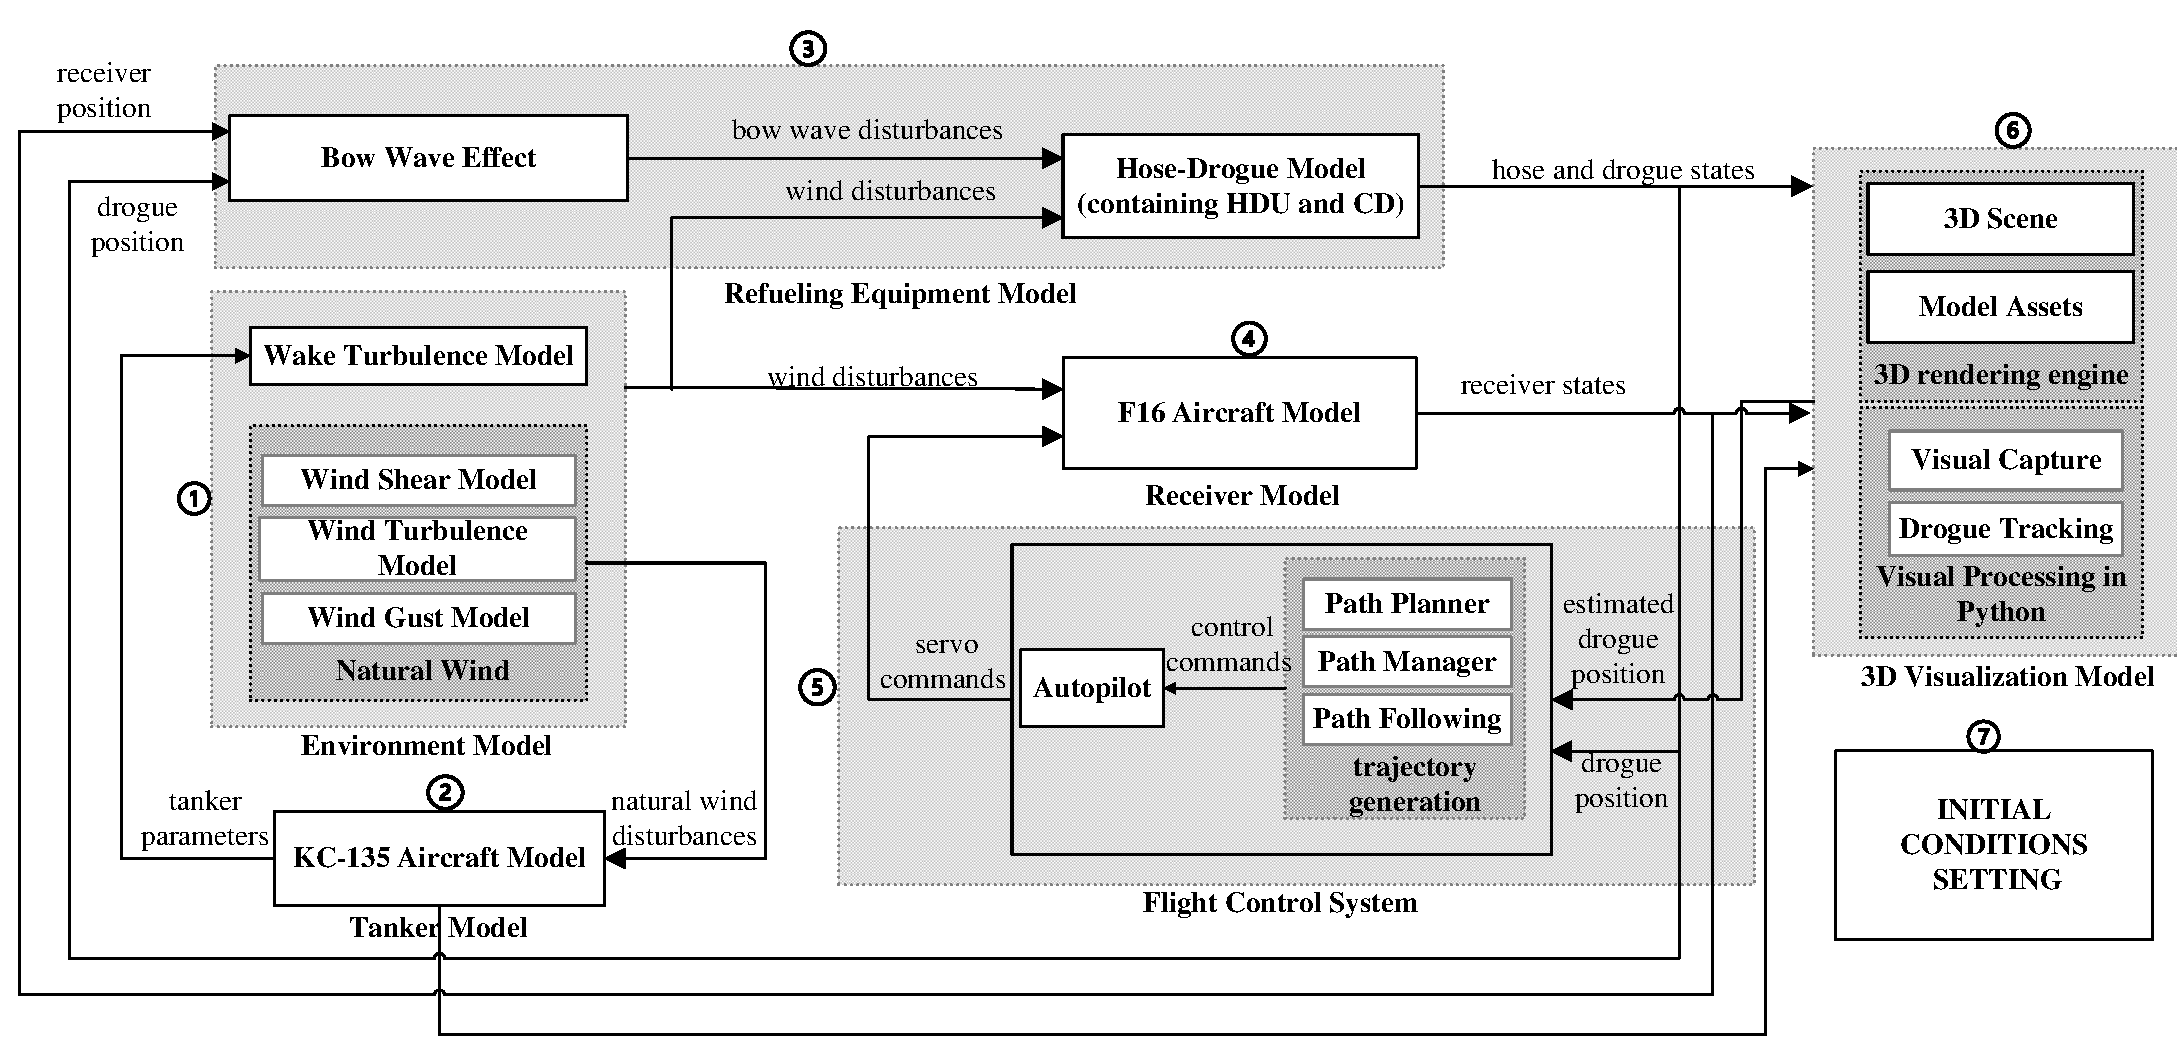
\includegraphics[width=1\textwidth]{Figures/Figs_Ch5/Fig2.pdf}
	\caption{The architecture of AARSim.}\label{FIG_2}
\end{figure}	

\section{AARSim framework }
\label{sec2}

\subsection{Architecture}\label{sec2.1}
A typical AAR system includes a natural wind model,  hose-drogue model,  receiver model,  tanker model, and flight control system. As shown in Figure \ref{FIG_2}, AARSim established in this paper contains all necessary subsystems.

\textcircled{1} Environment model

The block incorporates natural wind and wake turbulence caused by tankers, resulting in a vortex-induced wind field acting on the receiver aircraft. 

\textcircled{2} Tanker model

The tanker is supposed to be in steady flight mode. Hence the disturbances come from natural wind. Meanwhile, the tanker's states lead to wake turbulence.

\textcircled{3}	Refueling equipment model

The block contains a ``Bow wave effect" block, ``Collision Detection" (CD) block, and ``DRdynamics" block. The hose-drogue model is represented by a link-connected system. Precisely, a series of rigid links are adopted according to the finite element method to express the motion of the hose and drogue in the ``DRdynamics" block. By iteratively calculating each link's states (rotation and translation), the position and attitude can be determined at any moment. To avoid excessive contact with drogue and HWP mentioned above, an HDU model is adopted. Besides, the CD block can simulate the collision between the probe and the drogue. Furthermore, with the addition of the ``Bow wave effect" determined by the relative position of the receiver and drogue, an additional wind field would superpose the dynamics of the ``DRdynamics" block. 

\textcircled{4} Receiver model

The receiver is modeled as a 6-DoF rigid body, and the states are determined by translational and rotational kinematics and dynamics.

\textcircled{5}	Flight control system 

Receiver states are determined by the commands of its ``Flight control system" and the wind turbulence. The ``Flight control system" utilizes the estimated drogue position obtained by perception algorithms from the ``3D visualization model" to generate a trajectory for accomplishing autonomous rendezvous and docking. The true drogue position from the ``Refueling equipment model" can be used to assess the estimation accuracy and the controller performance.

\textcircled{6}	3D visualization model

The block provides typical scenarios associated with the refueling maneuvers and supports visual algorithms development for visual processing, including vision capture and drogue tracking.

\textcircled{7}	Initial condition setting

Many parameters need to be initialized before starting the AAR simulation process. The parameters can be di-vided into flight conditions, receiver and tanker status, hose-drogue status, and so on, which will be listed explicitly in Table \ref{Tab_2}.

\begin{figure}[th]
	\centering
	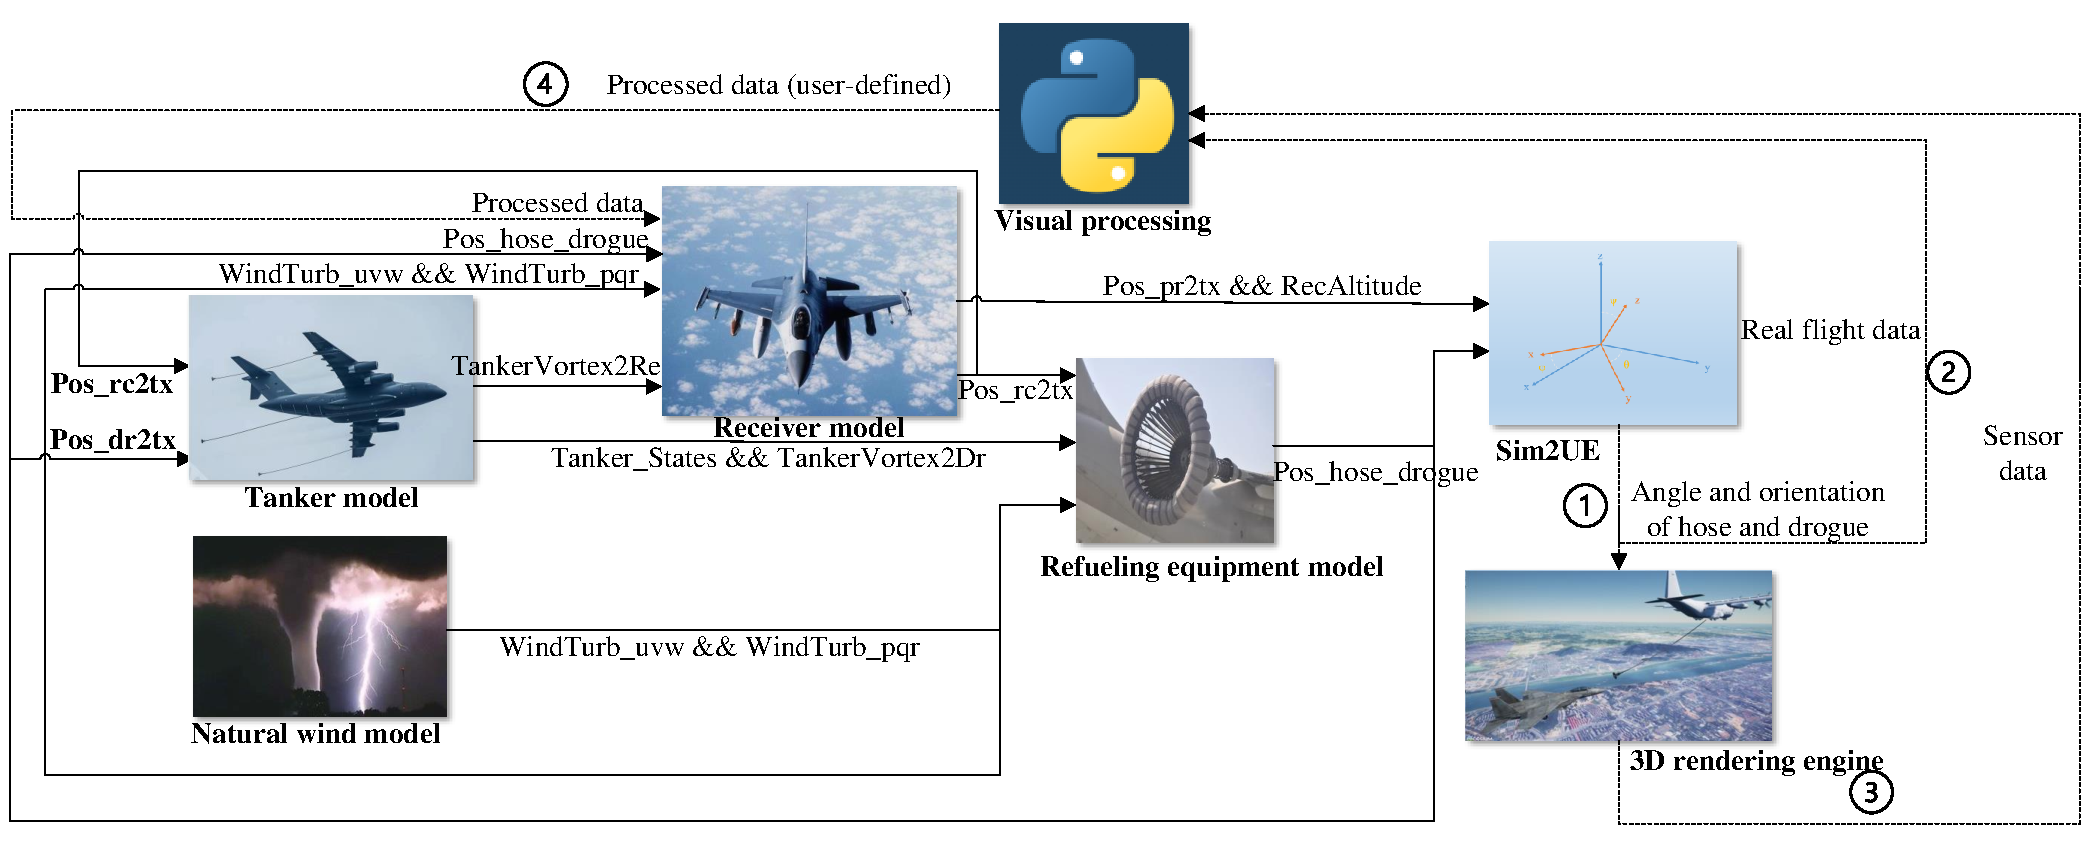
\includegraphics[width=1\textwidth]{Figures/Figs_Ch5/Fig3.pdf}
	\caption{The realization of AARSim.}\label{FIG_3}
\end{figure}

\subsection{Realization }\label{sec2.2}

A comprehensive toolbox is released to improve the efficiency of studies concerning AAR and to make re-searchers study further. As shown in Figure \ref{FIG_3}, the relationships among the receiver system, turbulence, and refueling equipment model are described clearly, which corresponds to Figure \ref{FIG_2}.

The complete toolbox's MATLAB$ ^{\rm{TM}} $/Simulink$^\circledR$ source code and experimental videos can be obtained in the following part of the paper. 

The dataflows of AARSim are displayed by solid lines and dashed lines which represent different natures in Figure \ref{FIG_3}.  The solid lines are the interior communication in Simulink$^\circledR$, while the dashed are the external communication among Simulink®, the 3D rendering engine, and Python.


$ \left( 1 \right) $ Solid line signals

The meanings of the signals are consistent with the dataflows among different blocks in Figure \ref{FIG_2}.

$ \left( 2 \right) $ Dashed line signals

The dataflows are separated into three parts.

\textcircled{1} Simulink$^\circledR$ $\longrightarrow$ 3D rendering engine

The information containing angles and orientations of models is sent to the ``3D rendering engine" to display.

\textcircled{2} Simulink$^\circledR$  $\longrightarrow$ Visual processing 

The real flight data is transmitted to the ``Visual processing" block to verify the information obtained by sensors. There are a total of 20 float types of data available. By setting the port address, users can send the real position and attitude of the tanker to Python.

\textcircled{3} 3D rendering engine $\longrightarrow$  Visual processing 

The sensors installed on the receiver can grasp information from the ``3D rendering engine" to process for further control. The information, such as images and depth, can be processed by some third-party vision libraries' functions when performing vision-in-the-loop for AAR simulation. 

\textcircled{4} Visual processing $\longrightarrow$ Simulink$^\circledR$

The processed data are sent back to Simulink$^\circledR$ for navigation. Specifically, the length of the processed data is set to 136 bits, the outputs are the ID of aircraft and the concrete data whose types are integers. In the vision-in-the-loop experiment, the output data are the estimated position of the drogue's central point calculated by user-defined vision algorithms, the distance of the depth camera mounted in the receiver, and the drogue's central point. The left 13 bits of data are reserved. 


\subsection{Interface usage }\label{sec2.3}

The usage of interfaces and the specific implementation of each model mentioned above are introduced in detail. Corresponding to Figure \ref{FIG_3}, they are introduced in order: natural wind model, tanker model, receiver model, refueling equipment model, and sim2UE \& 3D rendering engine \& visual processing.

\begin{figure}[th]
	\centering
	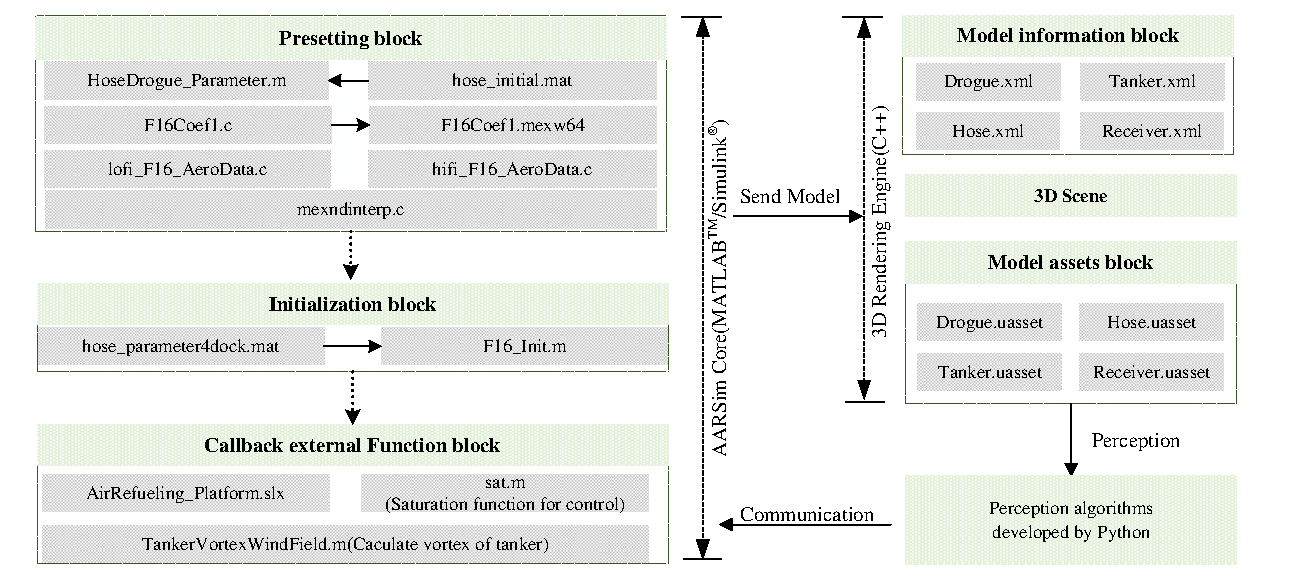
\includegraphics[width=1\textwidth]{Figures/Figs_Ch5/Fig4.pdf}
	\caption{Source code structure of AARSim.}\label{FIG_4}
\end{figure}

$ \left( 1 \right) $  Natural wind model 

The simulation incorporates both the Dryden model, which accounts for the effects of flight altitude and air-speed, and a discrete gust wind model that includes specific parameters such as time, amplitude, and length. The parameters in the natural wind model can be set to accommodate the AAR conditions.

$ \left( 2 \right) $ Tanker model

The calculation method of wake turbulence block generated by the tanker's vortex that influences the receiver and drogue's position is in the script file named ``TankerVortexWindField.m". 

$ \left( 3 \right) $ Receiver model

Wake turbulence, tanker vortex, and control instructions constitute the receiver's input. The ``Guidance" block and ``Controller" block are responsible for guiding and controlling the receiver to the demand position. The ``Controller" block contains two control schemes that support automatic controls via the LQR controller and manual control by handling a joystick connected to the simulation computer.

$ \left( 4 \right) $ Refueling equipment model 

The bow wave effect, which is determined by the relative distance between the drogue and the receiver, and the parameters of the receiver nose, can be obtained by the method of system identification\cite{wei2016drogue}. The ``HDU" block in ``DRdynamics" adopts the control method proposed in the previous work\cite{dai2019hose}. The ``Collision Detection" block takes the relative speed and position of the drogue and probe into consideration to generate force feedback which adopts a proportional controller to simulate the collision of the real docking process.

$ \left( 5 \right) $ Sim2UE \&\ 3D rendering engine \&\ Visual Processing 

Considering the initial parameters of the hose and drogue, the influence of wake turbulence, and the bow wave effect, ``Sim2UE" will calculate and send the position and attitude of each link of the hose and drogue to the ``3D rendering engine". The ``Visual Processing" block is used to develop perception algorithms, which consists of ``detect-realtime.py" for recognition and tracking, and ``Config.json" for settings. 

To introduce more explicitly, the source code structure and interaction of each part are shown in Figure \ref{FIG_4}. The programming environment is separated into three parts: ``AARSim Core (MATLAB$ ^{\rm{TM}} $/Simulink$^\circledR$ )", ``3D Rendering Engine (C++) ",c and ``Perception algorithms developed by Python". 

In AARSim Core, the ``Presettings block" has the parameters of the hose and aircraft model generated by the function previously. ``HoseDrogue\_\ Parameter.m" loads and processes the data of the hose from ``hose\_\ initial.mat" and then saves the data in ``hose\_\ parameter4dock.mat". The ``hose\_\ parameter4dock.mat" stories the parameters of hose, drogue, and HDU shown in Table \ref{Tab_2}. The file ended with ``.c"and ``. mexw64" are the settings of the receiver. 

Then, by running the initialization function `` F16\_\ Init.m" and ``AirRefuelingPlatform.slx" in order. The functions named ``TankerVortexWindField.m" and ``sat.m" is used during the simulation. The former is used to calculate the vortex of the tanker; the latter is utilized to generate control commands that incorporate saturation limits. 

\begin{figure}[!h]
	\centering
	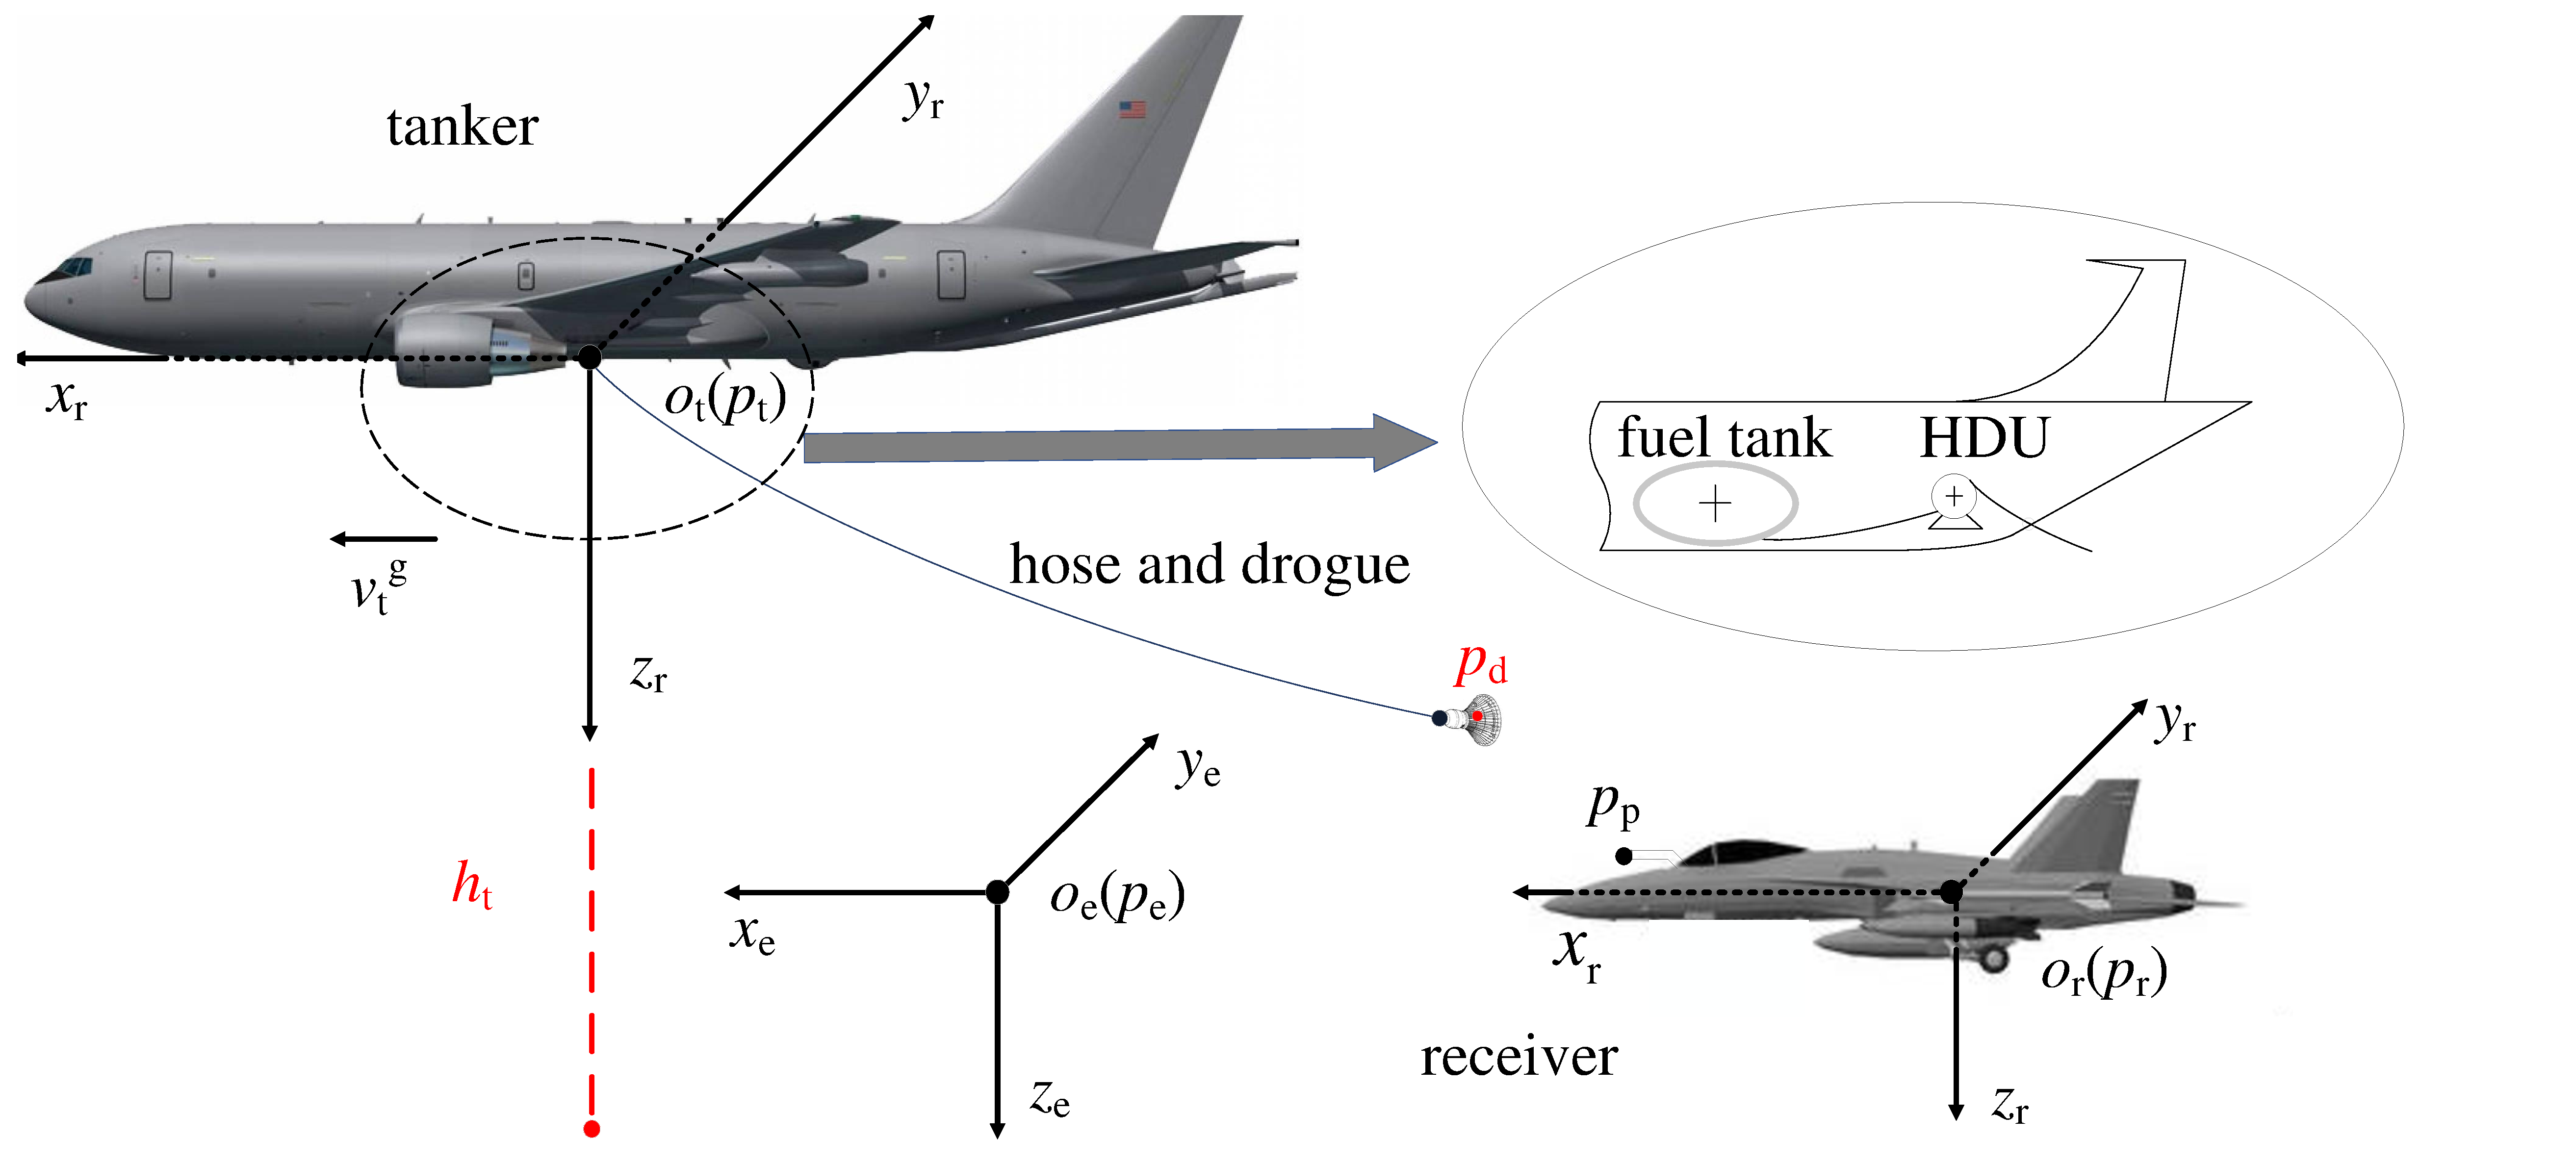
\includegraphics[width=0.9\textwidth]{Figures/Figs_Ch5/Fig5.pdf}
	\caption{Coordinate frames used in this paper and HDU unit.}\label{FIG_5}
\end{figure}

In ``3D Rendering Engine", the model assets and 3D scenes are pre-defined in the UE4 engine directory. The perception algorithms can be developed stand-alone to optimize the recognition results. The AARSim Core sends the model's position and orientation to the 3D Rendering Engine as well as perception algorithms. The 3D Render-ing Engine constructs a high-fidelity environment based on the information from MATLAB$ ^{\rm{TM}} $/Simulink$^\circledR$ and the model's properties, which can also be precepted by Python algorithms.

\section{AAR System Modeling }
\label{sec3}

As mentioned before, a typical AAR system should include the wind model, hose-drogue model, aircraft model, and flight control system, among which the receiver aircraft plays an essential role in probe-drogue refueling on account of performing a maneuver to accomplish rendezvous, formation with tanker aircraft as well as docking with the drogue. In this section, the design model of the AAR system is introduced in detail. For the convenience of building a mathematical model of every sub-system of the AAR system, the coordinate systems used in this paper are shown as follows (refer to Figure \ref{FIG_5}).

$ \left( 1 \right) $ Earth-Fixed 	Coordinate Frame  $\left( {o_{\rm{e}}} - {x_{\rm{e}}}{y_{\rm{e}}}{z_{\rm{e}}} \right) $: This frame is used to study the states of tanker and receiver aircraft relative to the surface of the earth, which is assumed to be flat. The $ {o_{\rm{e}}}{x_{\rm{e}}}$  axis is aligned with the projection of the velocity of the tanker $ {{\textbf{v}_{\rm{t}}^{\rm{g}}}} $ on the ground for convenience, and the $ {o_{\rm{e}}}{z_{\rm{e}}}$  axis points perpendicularly to the ground, and the $ {o_{\rm{e}}}{y_{\rm{e}}}$ axis is determined according to the right-hand rule.

$ \left( 2 \right) $ Tanker Coordinate Frame  $\left( {o_{\rm{t}}} - {x_{\rm{t}}}{y_{\rm{t}}}{z_{\rm{t}}} \right) $: This frame is used to study the states of receiver aircraft and hose-drogue relative to the tanker aircraft. The origin of this frame $ p_{\rm{t}} $ is fixed to the conjunctive point between the tanker and the hose. The $ {o_{\rm{t}}}{x_{\rm{t}}}$ axis is identical to the velocity of the tanker $   {{\textbf{v}_{\rm{t}}^{\rm{g}}}} $, and the $ {o_{\rm{t}}}{z_{\rm{t}}}$ axis points belly down, and the $ {o_{\rm{t}}}{y_{\rm{t}}}$ axis is determined according to the right-hand rule.

$ \left( 3 \right) $ Receiver Coordinate Frame $\left( {o_{\rm{r}}} - {x_{\rm{r}}}{y_{\rm{r}}}{z_{\rm{r}}} \right) $: This frame is used to study the states of receiver aircraft. The origin of this frame is fixed to the mass center of the receiver aircraft, namely $ {p_{\rm{t}}} $ . The $ {{o_{\rm{r}}}{x_{\rm{r}}}} $ axis points to the nose direction in the symmetric plane of the receiver aircraft, and the axis is in the symmetric plane of the receiver aircraft, pointing downward, which is perpendicular to the  $ {o_{\rm{r}}}{x_{\rm{r}}}$ axis, and the  $ {o_{\rm{r}}}{y_{\rm{r}}}$ axis is determined according to the right-hand rule.

\subsection{Aircraft model }\label{sec3.1}
\subsubsection{Tanker aircraft model }\label{sec3.1.1}

In an actual aerial refueling process, the tanker aircraft usually enters a racetrack orbit pattern to wait for rendezvousing with the receiver aircraft\cite{nato2013aerial}. Hence, it is felicitously assumed that the tanker aircraft maintains steady-state flight in a straight line with constant airspeed and altitude to simplify the problem without loss of generality. A KC-130 mass-point tanker aircraft model is used in our AAR platform with the flight condition of  h$ _{\rm{t}} $ = 3000 m  and  v$ _{\rm{t}} $ = 120 m/s   .
\subsubsection{Receiver aircraft model }\label{sec3.1.2}
The receiver aircraft used in the AAR platform is an F-16. The University of Minnesota puts forward a nonlinear F-16 aircraft model package, which is built on MATLAB$ ^{\rm{TM}} $/Simulink$^\circledR$ software including a low-fidelity model and a high-fidelity model with a more extensive aerodynamic data range, and leading-edge flap\cite{russell2003non}. The high-fidelity model has an additional control surface, namely the leading-edge flap, which is governed by the angle of attack, and the aircraft's static and dynamic pressures. It allows the aircraft to fly at higher angles of attack. Thus, the nonlinear F-16 aircraft model in the package is used as a receiver aircraft model in the AAR platform. The control input units and ranges of the F-16 aircraft model are shown in Table \ref{Tab_1}.

\begin{table}[th]
	\caption{Control input units and ranges of the F-16.}
	\renewcommand\arraystretch{1.3}
	\centering
	\begin{tabular}	
		[l]{lllll}
		\hline
		\makecell{Control \\ Input} & Units & Min Value & Max Value & Rate Limit  
		\\\hline 
		Thrust & lbs. &  1000  &  19000  &  $ ± $ 10000 lbs$ / $s  
		\\
		Elevator & deg. & $ -25 $ &  25  & $  ± $ 60 deg$ / $s 
		\\
		Aileron & deg. & $ -21.5 $ &  21.5  &  $ ±  $80 deg$ / $s 
		\\
		Rudder &  deg. & $ -30 $ &  30  & $ 30±120$ deg$ / $s 
		\\\hline
	\end{tabular}
	\label{Tab_1}
\end{table}

In AAR operation, the receiver aircraft with respect to the tanker's position and orientation rather than with respect to the earth-fixed frame is emphatically concerned, which indicates that it is necessary to model the re-ceiver aircraft in the tanker frame. It will be convenient to model the receiver aircraft in the receiver frame with a well-developed method and then transform it into a tanker frame.

The platform provides a mass-varying receiver model which is close to the actual AAR process. The mass of the receiver will increase with the amount of fuel added during the refueling process. The total weight and moment of inertia of the receiver will be influenced by the fuel tanker's change. The mass-varying receiver model ignores the refueling weight in the hose and the consumption, and it is only needed in the refueling phase which means the invariant mass receiver model can be utilized in the left phase of the AAR process. The force equations, moment equations, kinematic equations, and navigation equations of the invariant mass receiver model, and the detailed formulas derivation of the varying mass receiver model refers to Ref\cite{ma2018formation}.

\subsection{Refueling equipment model }\label{sec3.2}
In the probe-and-drogue system, there are usually two types to mount the central part of the refueling system on the tanker, including under the centerline, or using a pod under the wing. The centerline hose and drogue refueling is considered in AARSim, the wing-pod refueling can also be adopted. To suppress the hose whip behavior, the HDU utilizes a reel take-up system which is located in the front end of the flexible hose\cite{vassberg2003numerical} as shown in Figure \ref{FIG_5}. When fully deployed, the hose has a trailing length of  15 m , while a diameter of 0.068 m  and a specific linear density of  4.1 kg/m  is assumed. Besides, the high-speed drogue is modeled with a diameter of  0.70 m  and a weight of 29.5 kg .

A physically deduced multi-body model, namely the link-connected model, is used to describe the flexible hose-drogue dynamic model according to the finite element method, where the hose-drogue is regarded as ten rigid links. As shown in Figure \ref{FIG_6}, the orientation angles of each link with length  $ {l_j} \in \mathbb{R} $ are described by $ {\alpha_j} \in \mathbb{R} $ and $ {\beta_j} \in \mathbb{R} $ , where  $ j = 1,2, \cdots ,N $ and $  N \in {\mathbb{Z}^ + } $ is the number of rigid links (N $ =10 $ in AARSim). It is assumed that the masses and loads associated with each link are concentrated at the joints whose positions $ {P_j} \in {\mathbb{R}^3} $ 
And the drogue's position is expressed by $ P_{\rm{d}} $ . The effects of HDU and wind turbulence are also displayed in Figure \ref{FIG_6}. The resultant external force, including both gravitational and aerodynamic forces, acts on each lumped mass, whereas aerodynamic forces are due to the wake of the tanker, steady wind, and atmospheric turbulence. The drogue is modeled as a rigid body with a conical geometry and fine aerodynamics creating longitudinal and lateral forces, which is significant to respond realistically to the bow wave.

\begin{figure}[th]
	\centering
	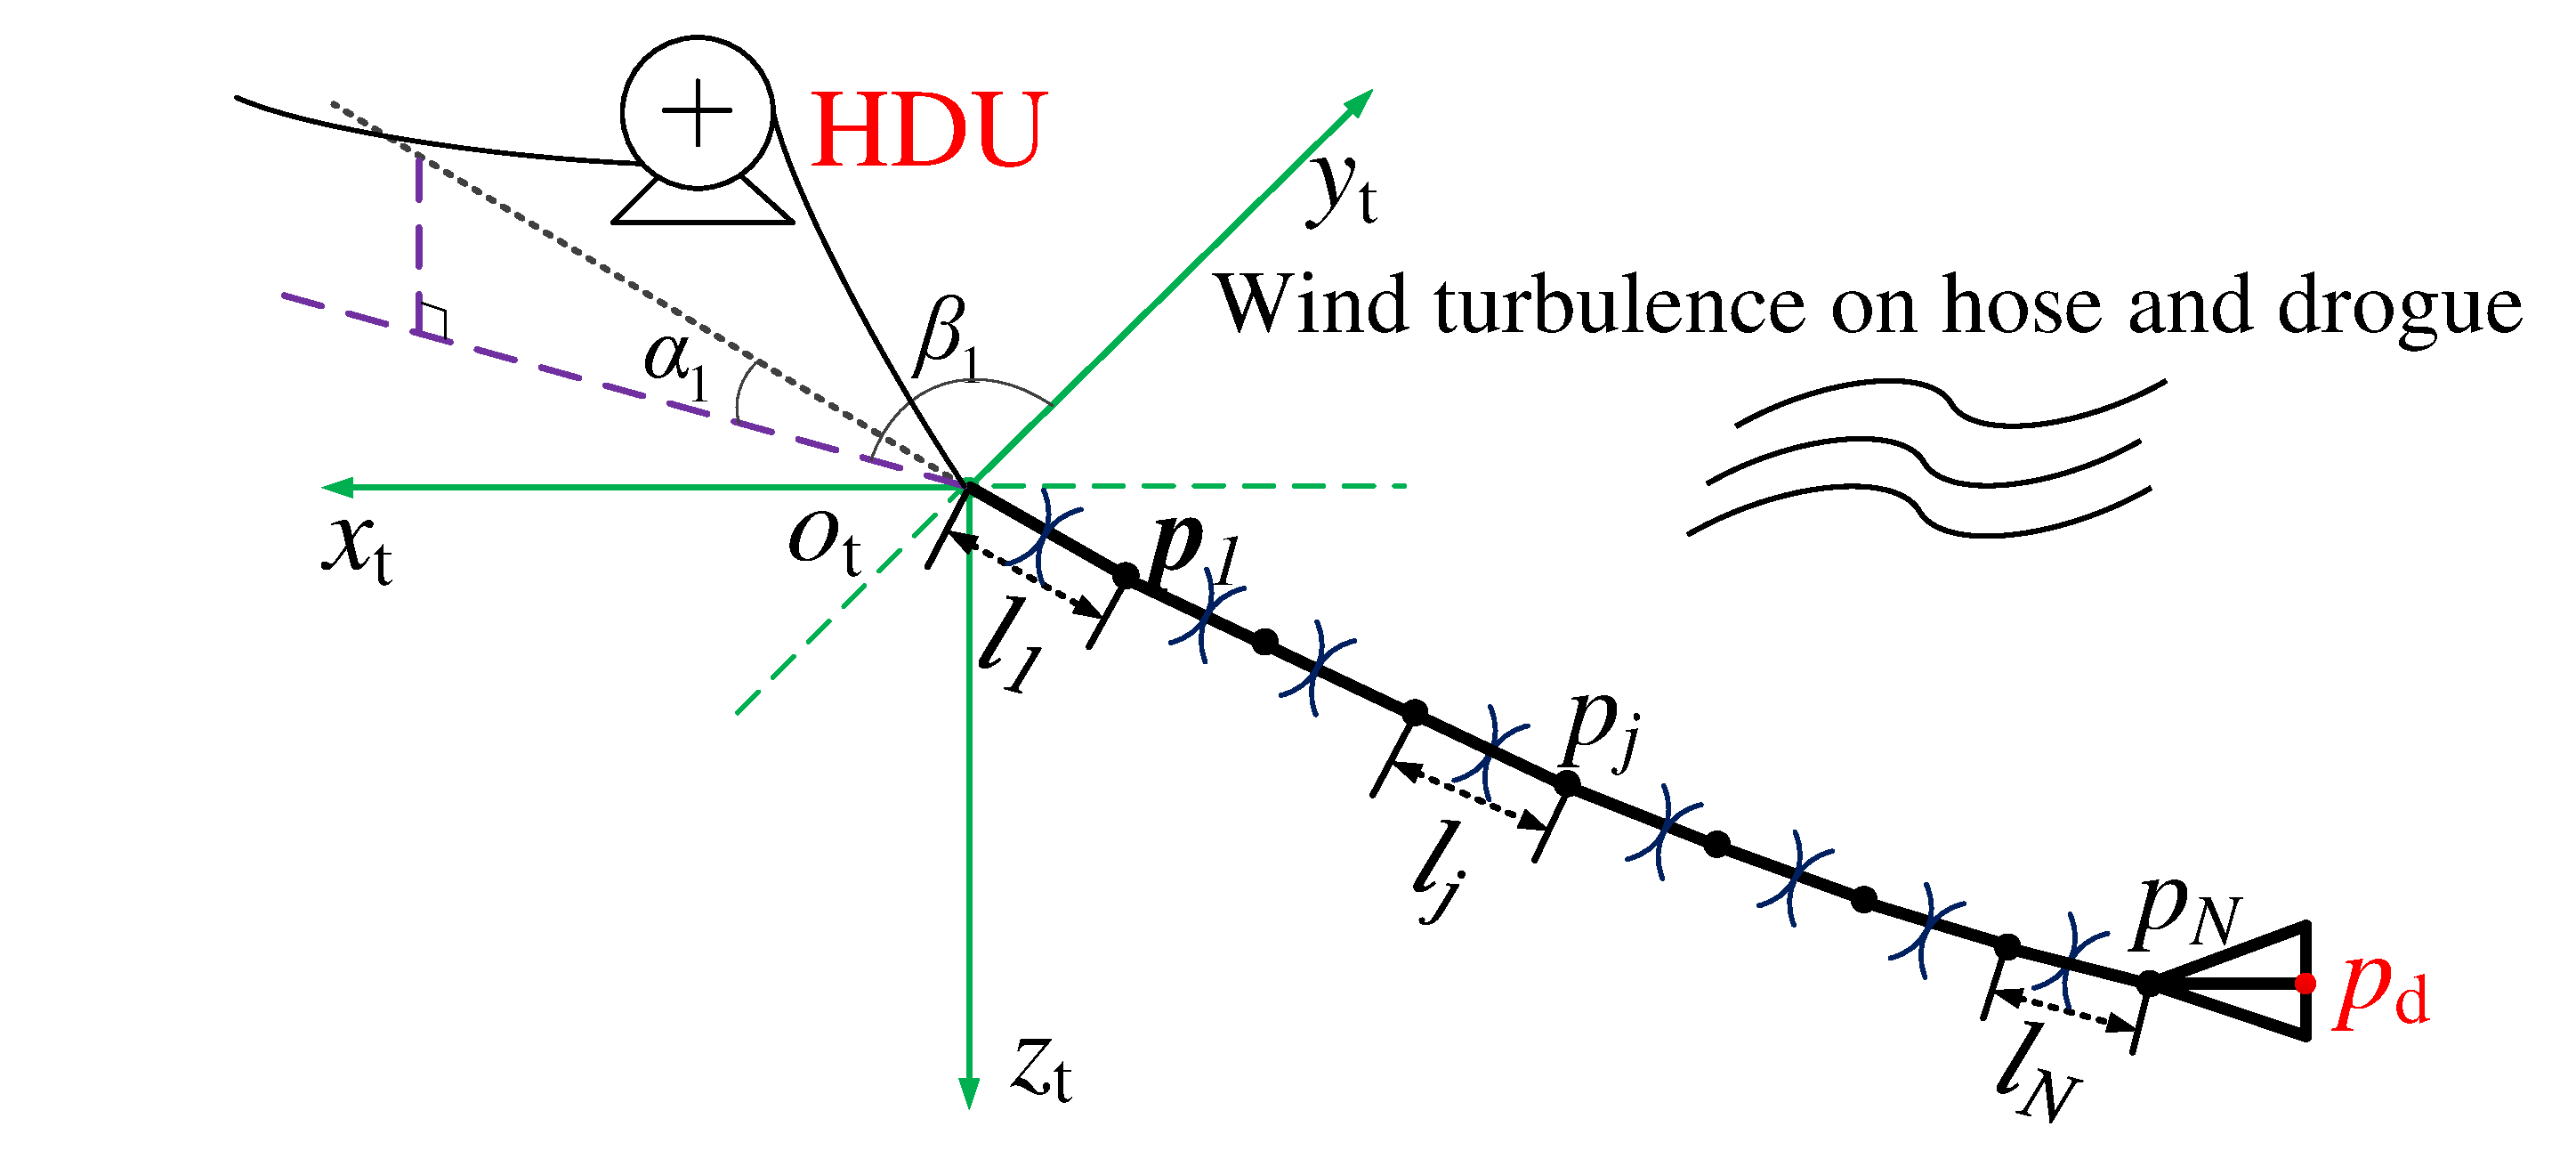
\includegraphics[width=0.6\textwidth]{Figures/Figs_Ch5/Fig6.pdf}
	\caption{The link-connected model of hose and drogue.}\label{FIG_6}
\end{figure}

The reel take-up system is used to retract the hose when hose tension drops below the static catenary value during drogue and probe coupling. To describe this scene, the link length is considered variable, which allows for studying the dynamic effects of the hose-drogue model, like hose whip behavior. However, for a reel take-up modeling purpose, only the first hose segment is modeled as having variable length. A modified HDU controller proposed in Ref.\cite{dai2019hose} based on Ref.\cite{vassberg2003numerical,ro2010modeling} has a good transient response.

\subsection{Natural wind model  }\label{sec3.3}
The air disturbance includes natural wind, wake turbulence of tanker, and bow wave, while bow wave only influences the hose-drogue model. What follows in this subsection will establish the natural wind model in detail.

\subsubsection{Natural wind }\label{sec3.3.1}
Wind turbulence and wind gusts are known as a part of perturbation that affects aircraft and refueling equipment seriously. Turbulence is a stochastic process defined by velocity spectra. According to the American Military Specification MIL-F-8785C\cite{moorhouse1980}, the Dryden wind turbulence model uses the Dryden spectral representation to add turbulence to the aerospace model by passing band-limited white noise through appropriate forming filters.

The turbulence intensities are determined from a lookup table that provides the turbulence intensity as a function of altitude and the probability of the turbulence intensity being exceeded. At altitudes between 1000 feet and 2000 feet, the turbulence velocities, and turbulence angular rates are determined by linearly interpolating between the value of low and high.                                                                                          

\subsubsection{Wake turbulence }\label{sec3.3.2}                                                                                                                                                                                                                                                                                                                                                                                                                                   
The vortices that trail from the tanker's lifting surfaces generate considerable turbulence for the receiver as well as probe-drogue, to which the Helmholtz horseshoe-vortex model is applicable\cite{thomas2014advances,dogan2005modeling}. The part of the vortex sheet along the span of the wing or horizontal tail is the bound vortex, whereas the parts that continue in the downstream direction are the tip vortices. Moreover, wing vortices rotate inward, and tail vortices rotate outward\cite{dogan2008flight} as shown in Figure \ref{FIG_7}. There is a total of six vortex filaments, including two bound vortices and four tip vortices. The velocity of the wind induced by the wake of the tanker at a given point is the vector sum from all six filaments.

\begin{figure}[th]
	\centering
	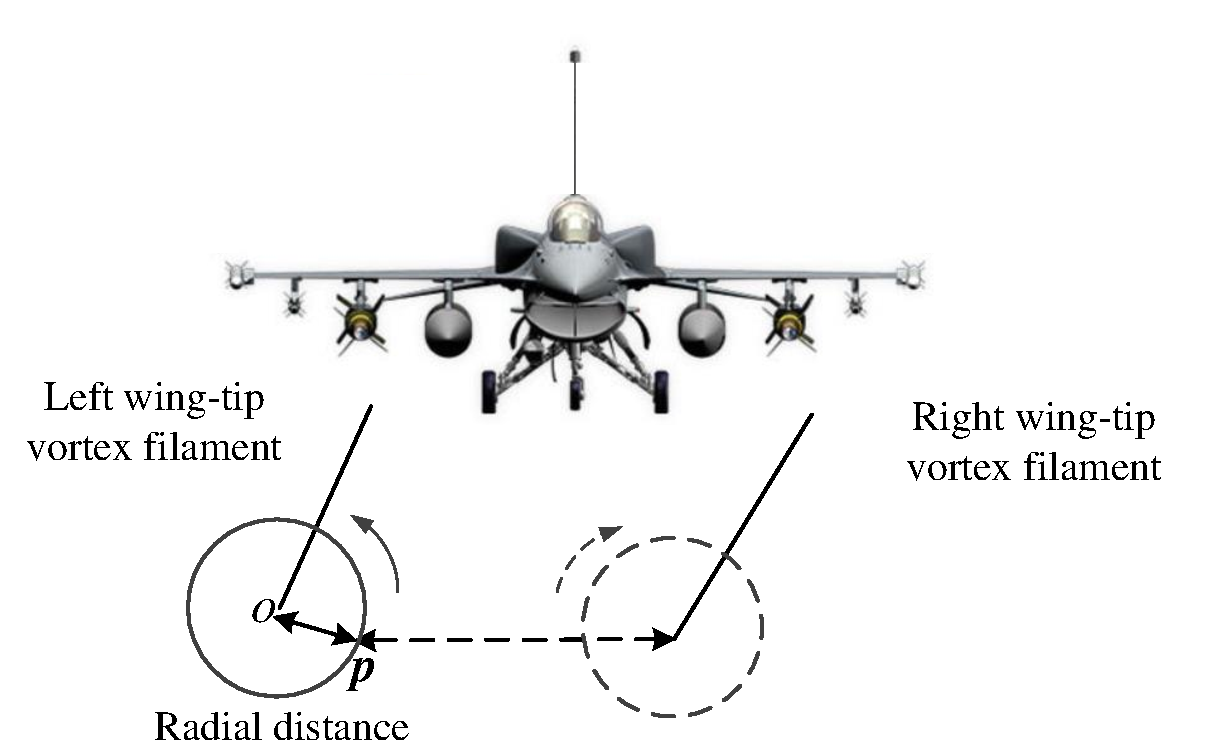
\includegraphics[width=0.6\textwidth]{Figures/Figs_Ch5/Fig7.pdf}
	\caption{Wing tip vortices induced by tanker aircraft.}\label{FIG_7}
\end{figure}

For a given point in wind axes, the velocity of the wind induced by the left-wing tip vortex can be computed by the vortex effect modeling technique\cite{dogan2008flight}.
\subsection{Bow wave effect }\label{sec3.4}
In a probe and drogue aerial refueling system, the bow wave of the receiver aircraft will produce a robust aerodynamic effect on the drogue at the docking phase. The bow wave effect occurs when the receiver aircraft approaches the drogue into the area of influence (AOI) of the bow wave effect, which is a significant difficulty of docking control in probe and drogue aerial refueling\cite{bhandari2013bow,dogan2013bow}. 

Two approaches are used to model the bow wave effect. The first approach represented in Ref\cite{dai2016modeling} can obtain an analytical form model which adopts stream function defined by the superposition of fundamental stream singulari-ties to model the inviscid flow field around the forebody of the receiver. Then the aerodynamic coefficients are used to calculate the induced aerodynamic force on the drogue. 

The other approach is represented in Ref\cite{wei2016drogue}.  where the bow wave effect model is figured out in the form of a nonlinear function vector with undetermined parameters based on profiles of training data within AOI which are obtained by Computational Fluid Dynamics (CFD) software, the undetermined parameters can be determined by nonlinear regression based on these training data. To work with the hose-drogue dynamic model, this bow wave effect model is suitable to simulate the behavior of the drogue with receiver aircraft approaching. Besides, this model applies to dock controller design to overcome the bow wave effect actively.

\subsection{Successful docking criterion  }\label{sec3.5}
During the refueling process, it is not easy for the receiver aircraft to contact the drogue. In addition, more serious is that the drogue occasionally causes damage to the receiver, such as cracked or broken canopies and damage to the probe. Therefore, the NASA AARD project\cite{dibley2007autonomous} represents a two-dimensional cross-section of the capture and miss criteria. A similar capture criterion of successful or failed docking attempts is defined in this platform. As shown in Figure \ref{FIG_9}, the capture radius $ R_{\rm{c}} $ is defined as 0.1m inside the outer ring of the drogue, which would reach a 90\%\  success rate with minimal vertical and lateral velocity, according to the recommendation of pilots.The success rate can also be predicted by the method proposed in Ref\cite{liu2020docking}.

A relative closing speed is required to capture successfully during the refueling scenario\cite{wei2016drogue}. Therefore, a successful docking attempt should satisfy
\begin{equation}\label{eq81a}%yinyong\eqref{eq*}
\begin{aligned} 
\begin{array}{l}
\sqrt {\Delta {y^2} + \Delta {z^2}}  < {R_C} {\rm{  }}\\
{v_{\min }} < {v_{{\rm{r}},x}} - {v_{{\rm{d}},x}} < {v_{\max }}    {\rm{ }}    	\quad	s.t. \  \Delta x = 0   
\end{array}
\end{aligned}
\end{equation}
where $ \Delta x $ , $ \Delta y $ and $ \Delta z $ represent the longitudinal, lateral, and vertical distance between probe and drogue; $ v_{{\rm{r}},{\rm{x}}} $ , $ v_{{\rm{d}},{\rm{x}}} $ are the longitudinal speed of the receiver and the drogue; and $ v_{\rm{min}} $ , $ v_{\rm{max}} $  are the minimum and maximum relative closing speed thresholds. The criterion\cite{dai2018iterative} implies that the radial error reaches within the capture radius, and the relative closing speed is within a range, indicating a successful docking attempt.  

\begin{figure}[th]
	\centering
	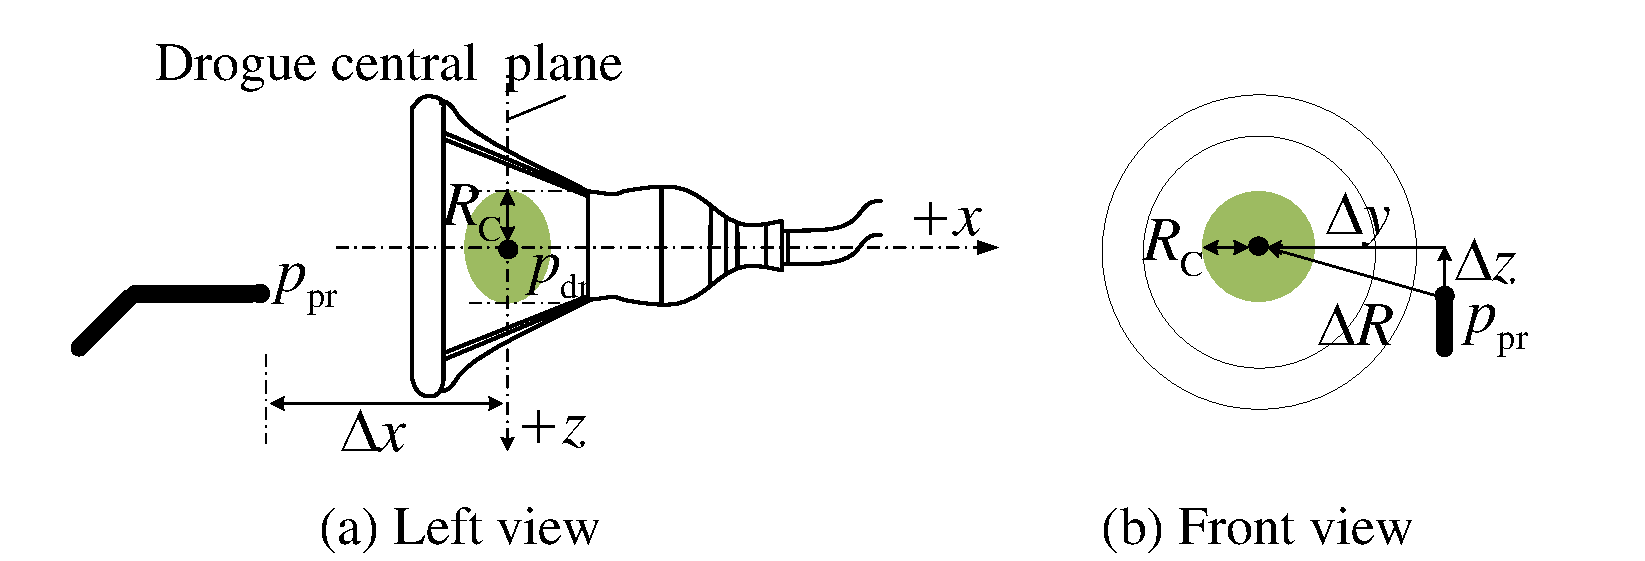
\includegraphics[width=0.6\textwidth]{Figures/Figs_Ch5/Fig9.pdf}
	\caption{Criteria of successful or failed docking attempt.}\label{FIG_9}
\end{figure}

When the docking phase starts, the simulation data will be recorded to calculate the docking errors while the demonstration running in the 3D rendering engine. Once the criterion set up for docking has been satisfied, the probe and the drogue will be connected to fly with relative static mode. The simulation can be paused and terminated manually or ends when the set time is up.

\subsection{3D visualization model }\label{sec3.6}
The simulation outputs are linked to a 3D rendering engine constructed by Unreal Engine 4 to provide typical scenarios associated with the refueling maneuvers. Such a 3D rendering engine can display real-time information of receiver, tanker, and hose-drogue within the simulation, which contains position, orientation, and attitude on the foundation of taking account of wind turbulence and bow wave effect. It also allows users to explicitly observe the relative relationships (position, etc.) among objects in the simulation and the whole dynamic docking process. Users can switch viewpoints at any time conveniently and observe the process of docking at any viewpoint to get the desired view of the scenarios. Figure \ref{FIG_10} shows three different views: side view, front view, and back view from Figure \ref{FIG_10}(a)-(c). Thus, the intuitive movement of the aircraft as well as the hose-drogue model is provided by the 3D rendering engine. Meanwhile, since the variety of the external environment is essential to the perception and control of aircraft, users can switch the scenarios in the 3D rendering engine to meet the actual needs of AAR.

The information is sent to the corresponding processing software through the transmission interface of the 3D rendering engine. The processing results can be transferred back to MATLAB$ ^{\rm{TM}} $/Simulink$^\circledR$ for control. A complete control closed loop is built, and users can develop and verify the aerial docking algorithms on this basis. Using the 3D rendering engine of the simulation platform can provide a high-fidelity display for the development and verification of the algorithm for aerial refueling. More importantly, the algorithm can be quickly iterated on the platform, which can significantly improve the development efficiency of the algorithm.

\section{Platform's function }
\label{sec4}
After modeling the AAR system, this paper will introduce the entire aerial refueling process, the initial settings, algorithms design, and model analysis in the platform.
\subsection{ AAR process}\label{sec4.1}
As shown in Figure \ref{FIG_11}, a typical AAR probe-drogue refueling procedure incorporates joining from the rendezvous position to the observation area where receivers enter an echeloned queue, and then the receivers maneuver to the astern of the tanker aircraft, namely the trail position in the designated refueling line which may be either the centerline or from a wing-mounted pod. Afterward, the receivers approach the drogue stably. Once refueled, the receiver disengages, falls back, and maneuvers starboard to the reform area. In general, there are five phases during the aerial refueling process: rendezvousing, formation-flying, docking, refueling, and reforming.

\begin{figure}[th]
	\centering
	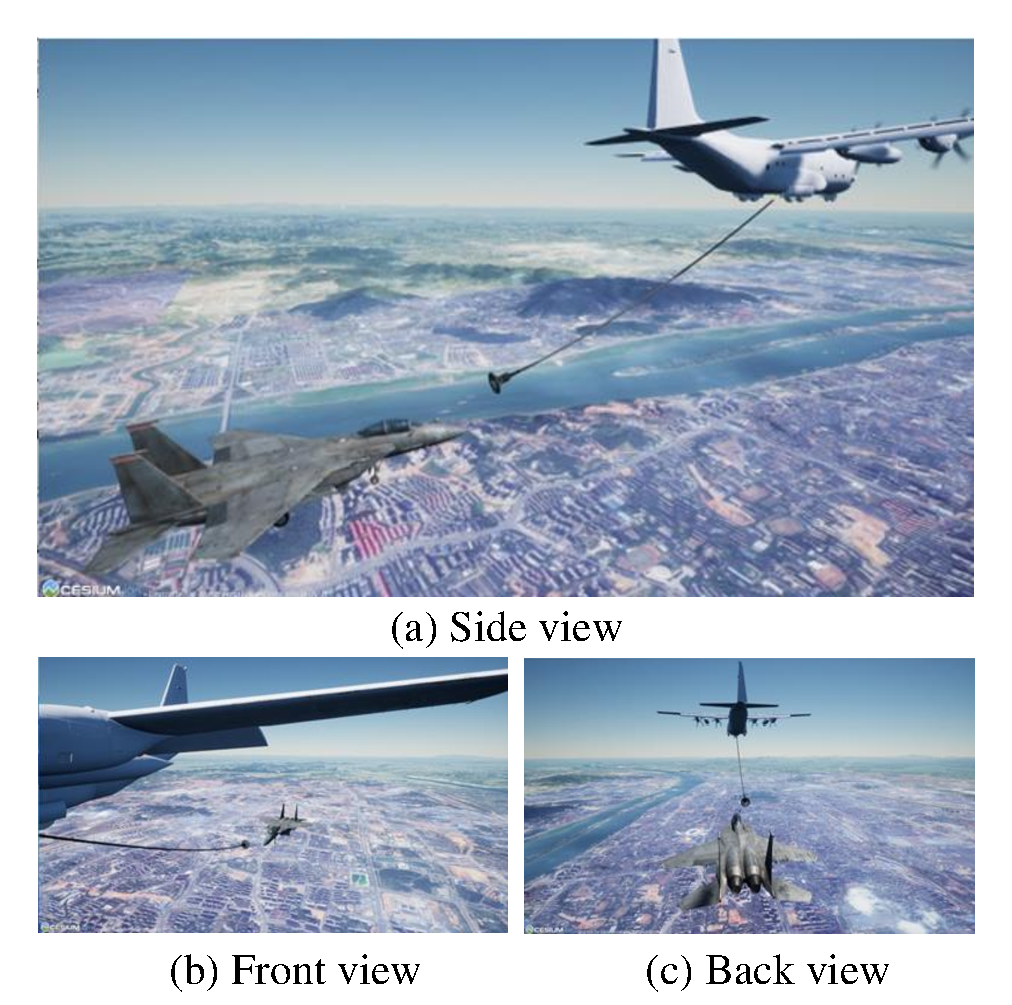
\includegraphics[width=0.5\textwidth]{Figures/Figs_Ch5/Fig10.pdf}
	\caption{Different viewpoints of the modeled virtual world.}\label{FIG_10}
\end{figure}

\begin{figure}[th]
	\centering
	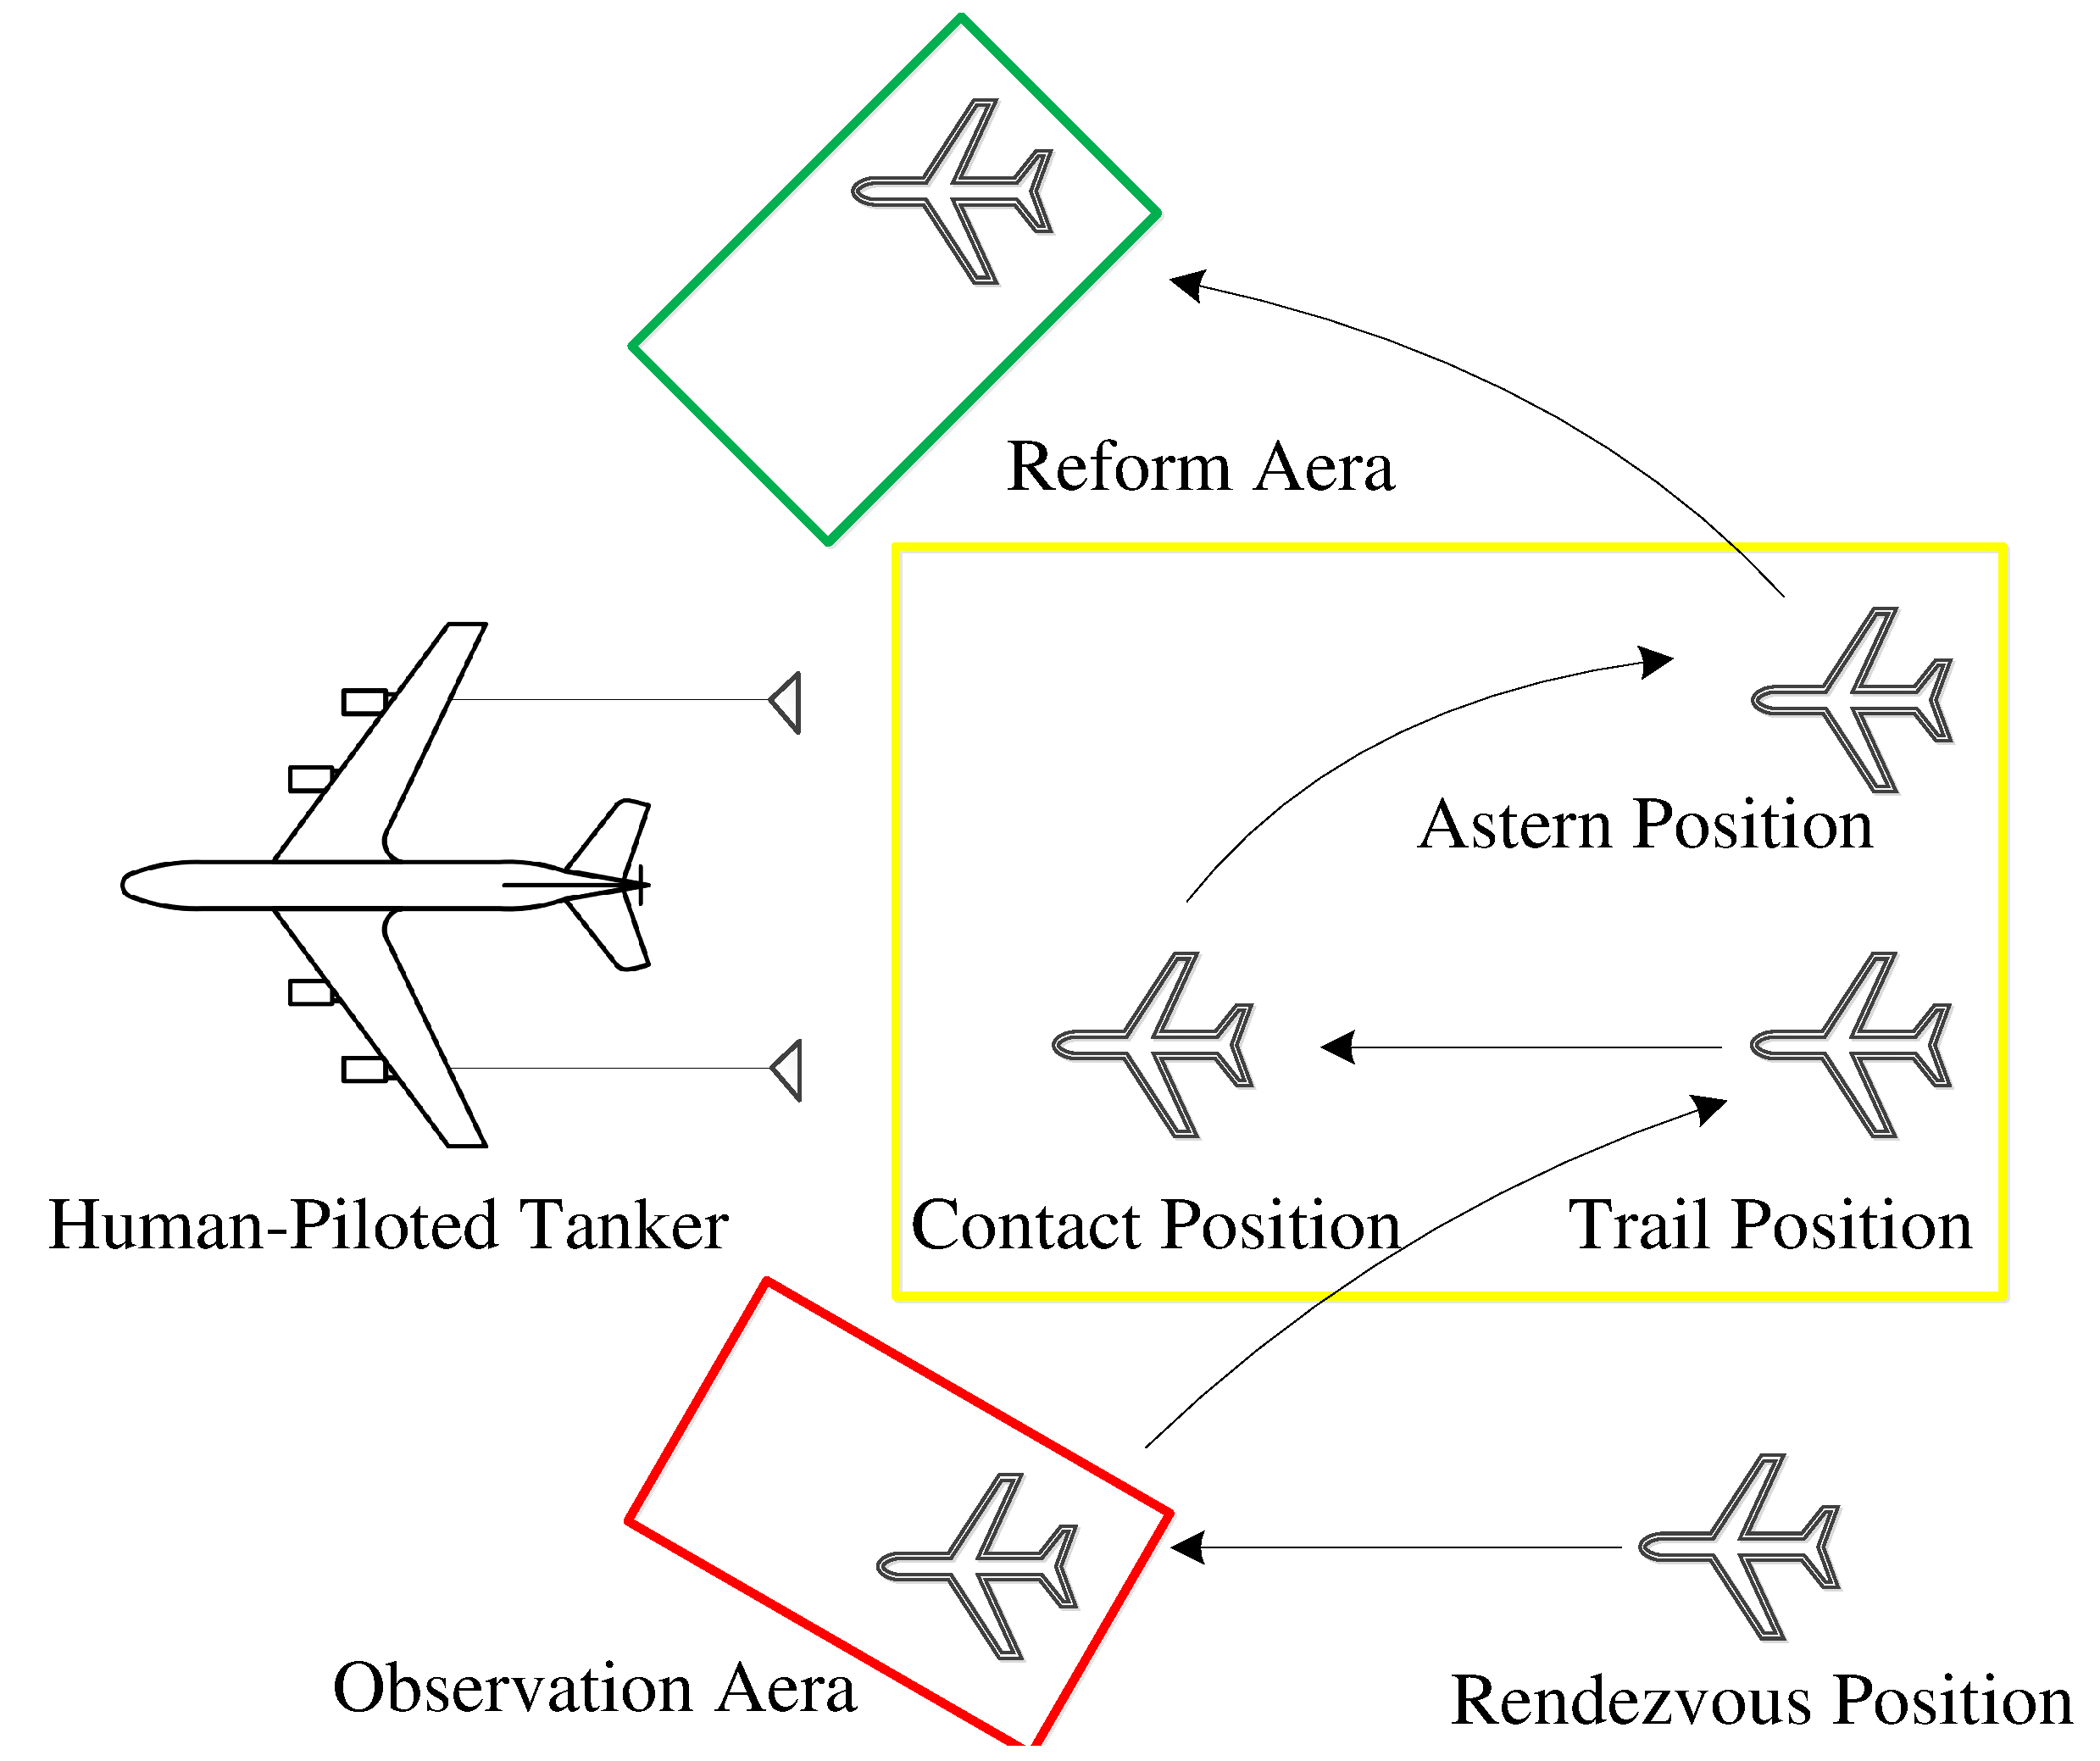
\includegraphics[width=0.6\textwidth]{Figures/Figs_Ch5/Fig11.pdf}
	\caption{Typical AAR refueling procedure.}\label{FIG_11}
\end{figure}

The built AAR platform can simulate these scenarios to provide a convenient way to study AAR. As previously mentioned, a complete aerial refueling process includes five phases. More precisely, several modes can be divided during the aerial refueling process, such as rendezvous mode, station-keeping mode, join mode, refueling mode, reforming mode, and so forth.
\subsection{ Initial condition setting}\label{sec4.2}
\subsubsection{Flight status }\label{sec4.2.1}
Some parameters should be initialized before starting the simulation. To be more specific, as shown in Table \ref{Tab_2}, many parameters can be defined by users to initialize the simulation environment which corresponds to the script file named ``F16\_\ Init.m". Take the linearized aircraft models as examples, the nominal conditions, including altitude and airspeed, are specific flight conditions of a tanker, around which the receiver aircraft is also linearized. Due to the nominal altitude of the tanker being  3000 m, the initial position of the tanker in the earth-fixed frame can be defined as 
$p_{{\rm{t}}0}^{\rm{e}} = {\left[ {\begin{array}{*{20}{c}}
		0&0&{ - 3000}
		\end{array}} \right]^{\rm{T}}}$, while the receiver's initial position is defined as 
$p_{{\rm{r}}0}^{\rm{e}} = {\left[ {\begin{array}{*{20}{c}}
		{ - 30}&1&{ - 2992}
		\end{array}} \right]^{\rm{T}}}$. Considering the relationship between the earth-fixed frame and the tanker frame, the receiver's initial position in the tanker frame represents the trail position at the docking phase.


\begin{table}[!th]
	\caption{ Initialized parameters with default values.}
	\centering
	\renewcommand\arraystretch{1.3}{
		\setlength{\tabcolsep}{5mm}{
			\begin{tabular}[c]{c|c|ccc}
				\hline
				\multicolumn{2}{c|}{{Parameters}} & {Symbol	in  ``F16\_ Init.m"} & {Default Value} & {Unit} 
				\\\hline 
				\multirow{2}{*}{Flight  Conditions} & nominal  altitude  & $ altitude  $ & 9843 & ft \\
				\cline{2-5}
				& Nominal airspeed & Airspeed & 393.72 & ft/s \\
				\hline
				\multirow{5}{*}{{Receiver}} & initial position & $ {p0\_ rc} $ & [-30 1 8]$ ^{\rm{T}} $ & m \\ 
				\cline{2-5}
				& attitude angle  & $ Euler\_ 0 $ & [0 trimAlpha 0] & rad  \\
				\cline{2-5}
				& angular velocity & $ pqr\_ 0 $ & [0 0 0]$ ^{\rm{T}}$ & rad/s  \\
				\cline{2-5}
				& probe position & $ d\_ pr\_ rc $ & [7.6 0.5 -2.44]$ ^{\rm{T}}$  & m   \\
				\cline{2-5}
				& weight & $ mass $ & 639.64  & slug \\
				\hline
				
				
				\multirow{3}{*}{Tanker} & initial position & $ xyz\_ 0 $ & [0 0 -3000]$ ^{\rm{T}}$ & m\\
				\cline{2-5}
				& wingspan & $ wingspan $  & 40 & m \\
				\cline{2-5}
				& weight & tankerWeight  & 8000 & kg \\
				\hline
				
				
				
				
				
				\multicolumn{2}{c|}{{Parameters}}  & \makecell{Symbols in \\ ``hose\_\ parameter4dock.mat"} & Default Value & Unit \\
				\hline
				\multirow{3}{*}{Drogue} & drag coefficient & $ Cdr\_\ $  & 0.8 & - \\
				\cline{2-5}
				& weight & $ Mdr $  & 29.5 & kg \\
				\cline{2-5}
				& radius & $ Rdr $  & 0. 305 & m \\
				\hline
				
				
				\multirow{6}{*}{Hose} & number of links & $ N $ & 10 & - \\
				\cline{2-5}
				& length & $ length $ & 15 & m  \\
				\cline{2-5}
				& linear density & $ I\_\ density $ &  4.1 & kg/m    \\ 
				\cline{2-5}
				& linear radius (external) & $ RI $   & 0.0336 & m  \\
				\cline{2-5}
				& radius (internal) & - &  0.0254 & m    \\ 
				\cline{2-5}
				& length of first link & $ I1 $ &  2 & m    \\ 
				\hline
				
				\multirow{3}{*}{HDU} & coefficient & $ k\_\ reel $ & 0.5 & - \\
				\cline{2-5}
				& coefficient & $ kd $ & 500 & - \\
				\cline{2-5}
				& Static tension    force & $ T\_\ reel\_\ initial $ & 1610 & N \\
				\hline
				Criteria & capture radius & - & 0.15 & m
				\\\hline
				
				
	\end{tabular}}}\label{Tab_2}
\end{table}

Parameters listed in Table \ref{Tab_2} are dependent on the model's materials such as the drag coefficient of the drogue, linear density, and radius of the hose; or specifications like the receiver's probe position, the tanker's wingspan and weight. Drogue's parameters left are predefined by the models themselves. 

The number of links can be adjusted by modifying the block in the simulation. If users want to adjust the length and the first link's length, change them in an initialization file. The parameters in HDU can be adjusted without constraints as long as it works better. The constrained parameters are nominal altitude, nominal airspeed, and trim-states of the receiver. The nominal altitude and airspeed are supposed to match the aircraft's performance, and the trim state can be set for specific conditions according to users' demands. 
\subsubsection{Sensors }\label{sec4.2.2}
Multiple types and numbers of sensors are supplied for the perception of AAR in the platform. As shown in Figure.\ref{FIG_3}, the installation of sensors can be initialized in the perception algorithm when constructing the communication with Simulink$^\circledR$. To recognize and locate the drogue, the receiver needs to mount various sensors to get relevant information such as an RGB camera for color images and a depth camera for distance. At the same time, the types of sensors mounted on the receiver vary according to different conditions. For example, the infrared camera is applied in a situation that lacks visible light. If a more accurate perception is needed, point cloud data obtained by Light Detection and Ranging (LiDAR) is also available. The sensors' effects of depth image and RGB image are shown in Figure \ref{FIG_12}. Particularly, the darker the black, the closer the distance is in Figure \ref{FIG_12}(a).

\begin{figure}[th]
	\centering
	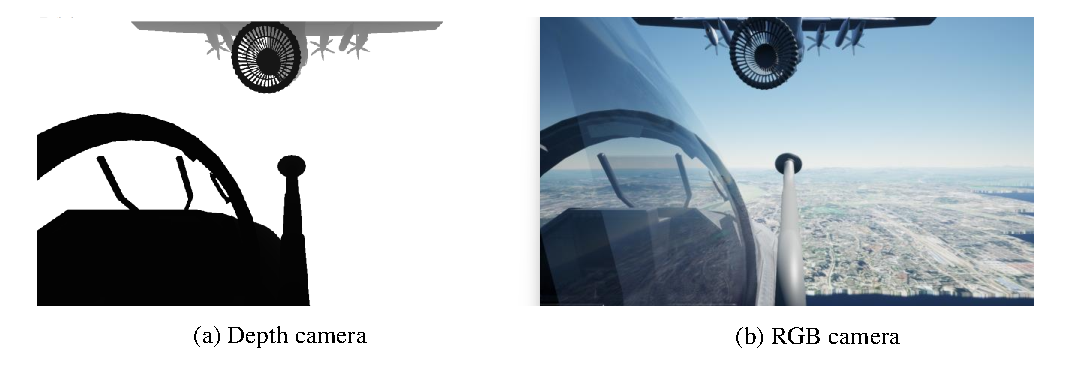
\includegraphics[width=1
	\textwidth]{Figures/Figs_Ch5/Fig12.pdf}
	\caption{Images obtained by sensors.}\label{FIG_12}
\end{figure}

\subsubsection{3D Scenarios and model assets }\label{sec4.2.3}
As shown in Figure \ref{FIG_13}, external environment conditions are essential to the perception and control of aircraft during the AAR process. The scenarios cover wide areas to satisfy long-distance experiments. Users can switch different AAR scenarios and develop user-defined scenarios in the 3D rendering engine. In addition, real satellite imagery scenes can be introduced if needed.

Model assets can also be replaced so users can select proper models of aircraft or place markers on drogue and flexible hose models for recognition in the UE4 engine which corresponds to the Model assets part in Figure \ref{FIG_4}. AARism provides maps such as ``3D Display", ``Mountain Terrain", ``Mountain Road" and ``Changsha" which correspond to  Figure \ref{FIG_13}(a)-(d) respectively. Users can switch different maps when entering the 3D visualization model by inputting the key ``M". 

\begin{figure}[th]
	\centering
	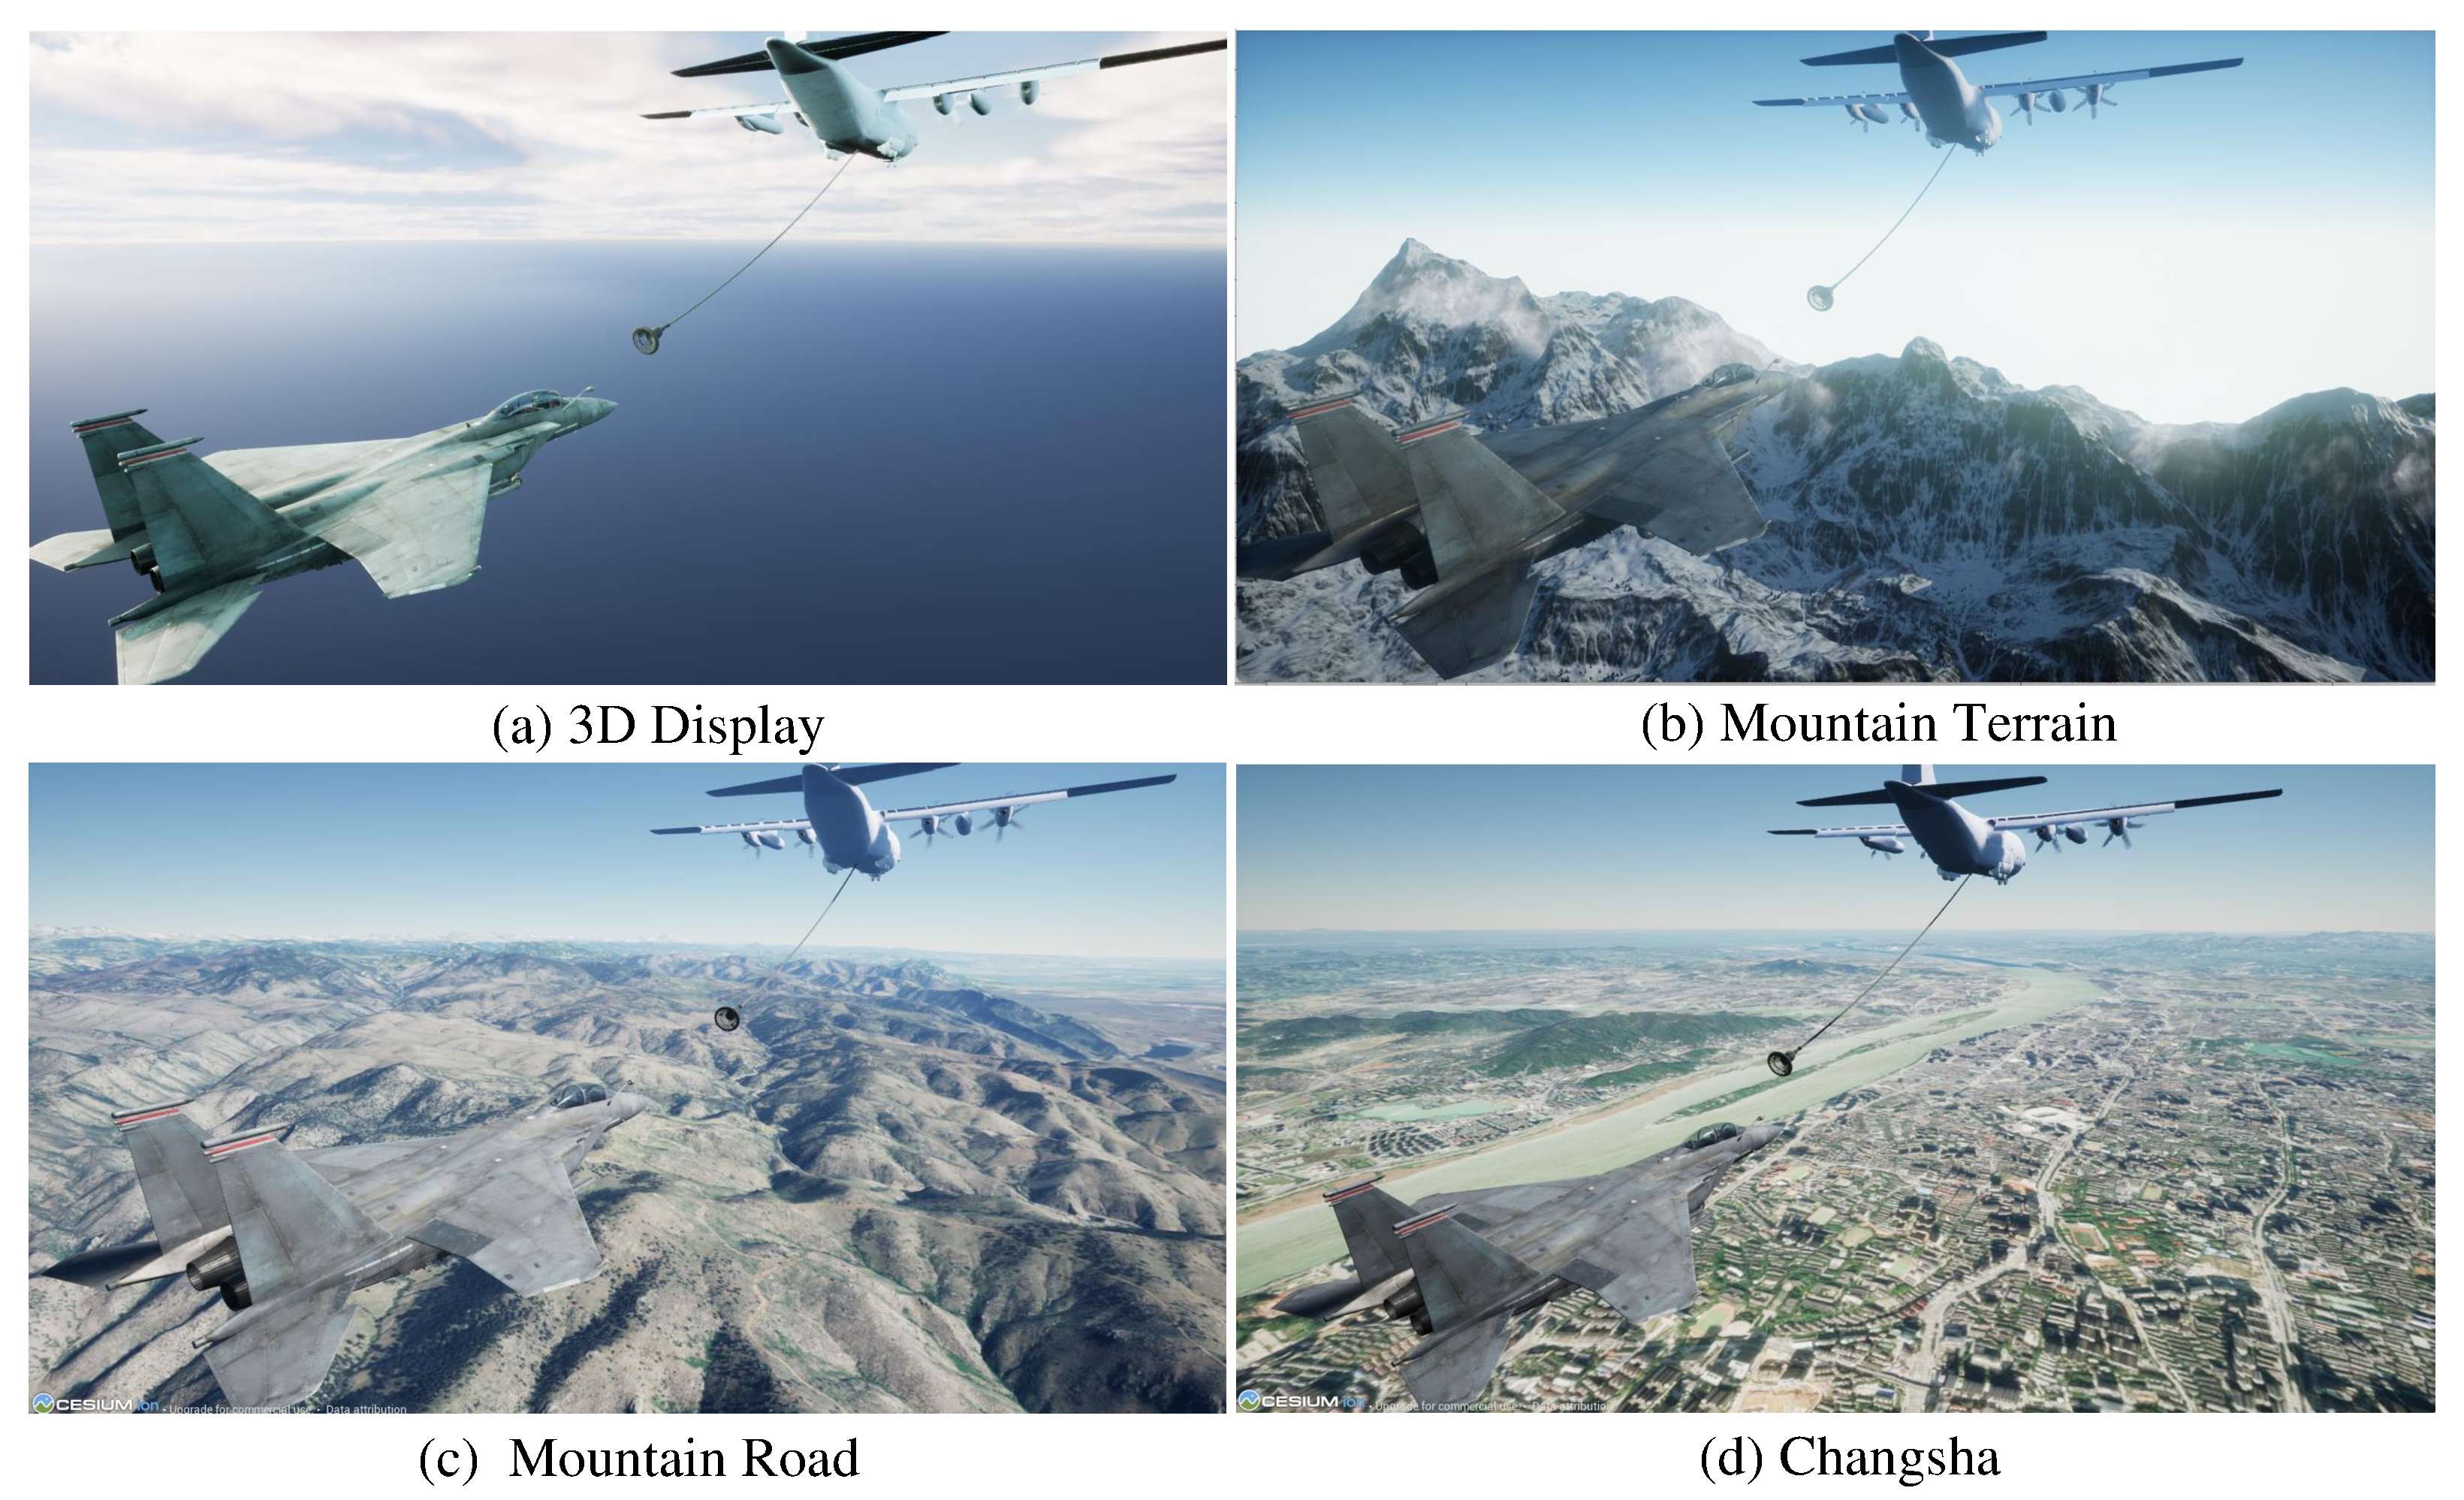
\includegraphics[width=0.9\textwidth]{Figures/Figs_Ch5/Fig13.pdf}
	\caption{Scenarios of AAR.}\label{FIG_13}
\end{figure}


\subsection{Algorithm design}\label{sec4.3}
\subsubsection{Navigation algorithm}\label{sec4.3.1}
The drogue's position needs to be recognized precisely for docking during the process. Therefore, the navigation algorithm designs are fundamental and significant tasks that rely on the data obtained by sensors. The platform supports the perception algorithms' development and deployment in the ``3D visualization model". As mentioned above, communication has been established between Simulink$^\circledR$ and Python which can be used to transmit information generated by the user-designed vision algorithms. Due to the diversity of sensors' data, users can determine certain or multisensory fusion perception algorithms.
\subsubsection{Guidance algorithm}\label{sec4.3.2}
The development of a guidance algorithm has a close relationship with the navigation algorithm. The interface of visual capture and drogue tracking is provided to design the navigation algorithms that control and navigate the aircraft's flight. The Python block in Figure \ref{FIG_3} obtains the information collected by sensors in the 3D rendering engine, and then the drogue's position is calculated by the vision algorithms and sent back to Simulink$^\circledR$ for guidance and control. In the vision-in-the-loop experiment, the processed data from Python can be added to the navigator block to improve the performance of the AAR, which fully demonstrates the practicability and extensivity of the platform.
\subsubsection{Control algorithm }\label{sec4.3.3}
Different controllers must be designed to meet various task requirements, or the controller parameters must be changed to accommodate various conditions. A position-tracking controller can guide the receiver to the target location by following the generated reference trajectory when the receiver plans to maneuver from the rendezvous position to the observation area or from the observation area to the trail position. In contrast, it probably does not apply to docking control because of the severe air disturbance, especially the bow wave effect acting on the drogue at the docking phase. Therefore, an interface is provided for designing the controller to achieve a different task in the AAR simulation platform. 
\subsection{Model analysis  }\label{sec4.4}

According to the initial settings and algorithm designs, the analysis concerned system stability and periodicity, station-keeping controller, wind disturbance, HDU controller, and docking accuracy can be implemented. Table \ref{Tab_3} shows the crucial parameters to analyze in ``F16\_\ Init.m". Users can exert a pulse signal to the system to observe the outputs of the system to analyze the system stability and motion mode as well as the station-keeping controller's performance. The analysis of wind turbulence and HDU controller is recommended to record the data while running.

\begin{table}[th]
	\caption{ Analysis parameters.}
	\renewcommand\arraystretch{1.3}
	\centering
	\begin{tabular}	
		[c]{cccc}
		
		\hline
		Analysis item & Parameter1  & Parameter2 & Parameter3  
		\\\hline
		\makecell{Stability \\ motion mode} & $ A\_\ lon $ & $ B\_\ lon $ &$  C\_\ lon\_\ xd\_\ h $
		\\
		\makecell{station-keeping  \\ controller} &$  k\_\ lon $ & $ k\_\ la $ & -
		\\
		\makecell{wind \\ turbulence} & \multicolumn{3}{c}{{\makecell{$ The\  parameters\  are \ in$ \\ $``Total\  Turbulence"\  block $}}}
		\\
		\makecell{HDU \\ controller} & $ T\_\ hose $ & $ dl\_\ 1 $ & -
		\\\hline
	\end{tabular}
	\label{Tab_3}
\end{table}

The parameters of the receiver's state space equation are listed in ``F16\_\ Init.m". Take the longitude equation as an example to analyze the stability and motion mode, the parameters are ``A\_\ lon", ``B\_\ lon" and ``C\_\ lon\_\ xd\_\ h". The station-keeping controller is designed as an LQR controller, the parameters are ``k\_\ lon" and ``k\_b\ la" which represent the feedback of longitude and lateral direction respectively. Attention must be paid to the ``Total Turbulence" in block ``Refueling equipment model" to analyze the wind turbulence. For the HDU controller, ``Tu\_\ hose" and ``dl\_\ 1"m are the tension and the slack rate of the hose after running the simulation. 

\section{Demos  }
\label{sec5}
\subsection{Demo objectives}\label{sec5.1}
Objective 1: The first demo will demonstrate the complete process of using the platform to simulate AAR. A vision navigation method is adopted to recognize the drogue and perform docking tasks considering the error of satellite navigation signals and the dynamic characteristics of the drogue in close range. The initial settings, algorithm design, results, and analysis will be introduced in detail. As shown in Figure.\ref{FIG_8}, the entire AAR task is performed in this section. 

Objective 2: To enhance the effectiveness of pilot training on the ground, AARSim provides support for both automatic and manual control using a joystick connected to the simulation computer. Objective 2 is similar to Objective 1, but it replaces the LQR controller of the ``Controller" block with a physical joystick in the receiver model as shown in Figure \ref{FIG_3}. This feature can provide a more realistic flight simulation environment, which can aid pilots in becoming more familiar with the aircraft's operation and help them develop their emergency response skills. The joystick control interface is open, allowing users to design the transfer function of the joystick's input.

\subsection{Initial settings}\label{sec5.2}
The setting of flight status is consistent with the default values in Table \ref{Tab_2}, as shown in Figure \ref{FIG_14}(a). In Figure \ref{FIG_14} (b), an RGB camera and a depth camera are selected to mount on the receiver to capture images and depth in-formation during AAR. The sensors' parameters such as type, location, and angle of installation are set in advance in ``Config.json" which will be utilized to initialize sensors when the navigation algorithm starts. The model assets and scenarios are kept as default.

\begin{figure}[th]
	\centering
	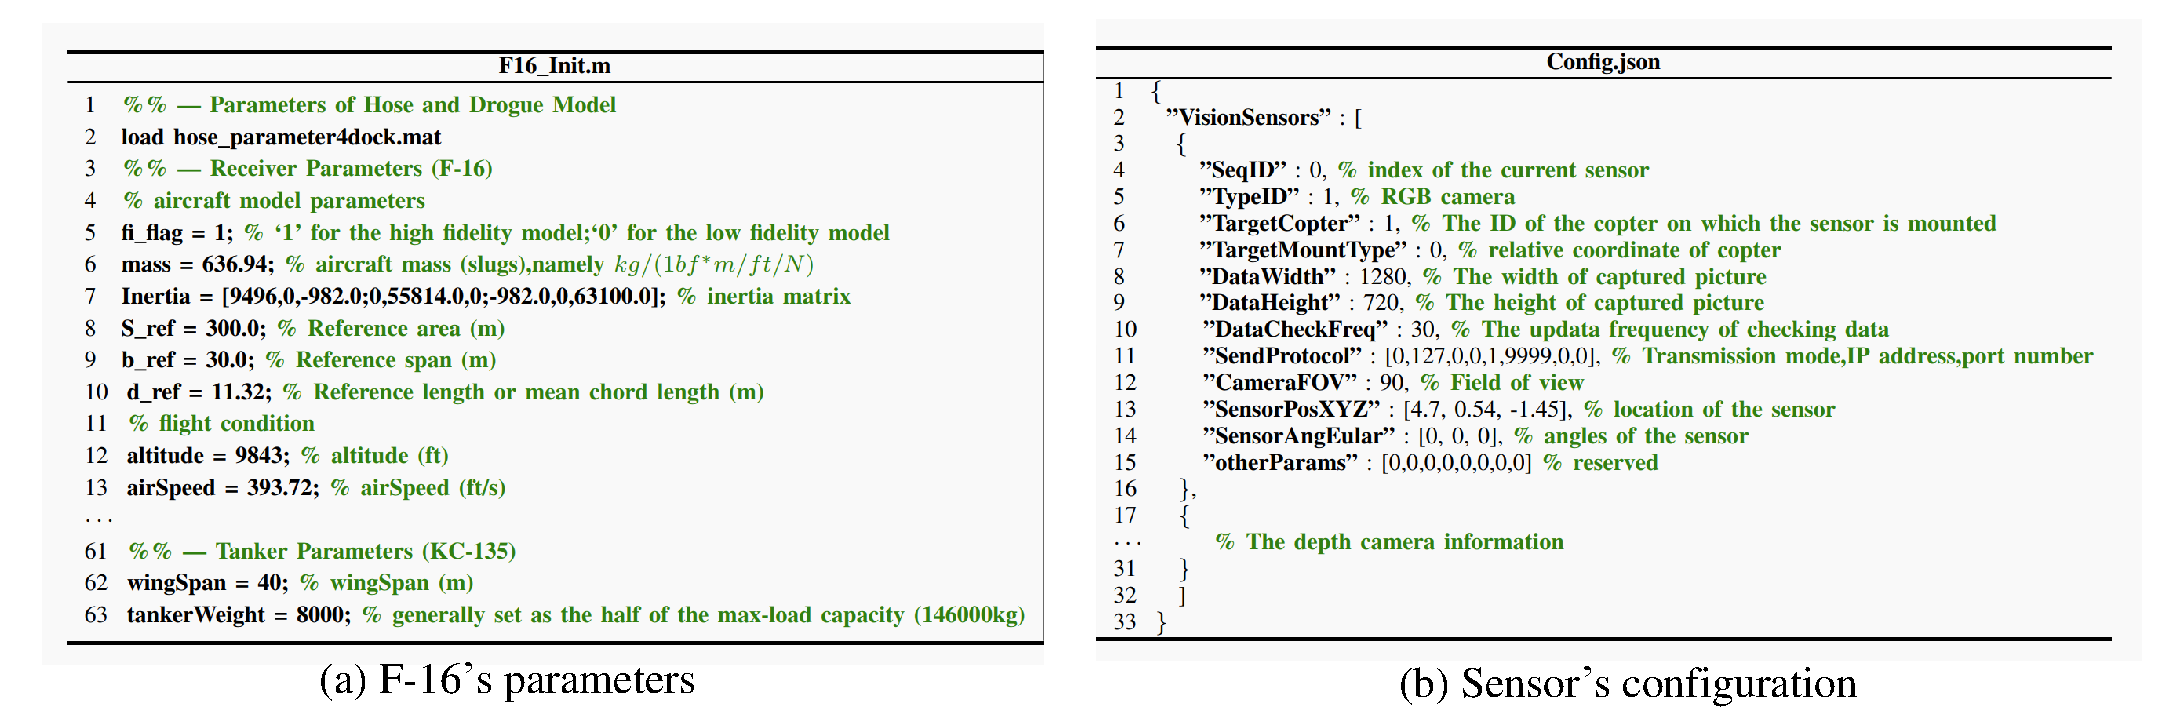
\includegraphics[width=1\textwidth]{Figures/Figs_Ch5/Fig14.pdf}
	\caption{Initialization files.}\label{FIG_14}
\end{figure}

\subsection{Implement of two objectives}\label{sec5.3}
The built platform can realize typical aerial refueling tasks, such as station keeping, docking control, and joining from the rendezvous position to the observation area, with a nonlinear aircraft model. 

Researchers who pay attention to the design of linear models can also deploy concerned algorithms in the platform. A linearized model is introduced in this part for controller design. After trimming the nonlinear equation, linearizing the nonlinear model at a steady level flight condition $ \left( {{\bf{X}}_{\bf{r}}^{\bf{*}},{\bf{U}}_{\bf{r}}^{\bf{*}}} \right) $, and letting $  
{\tilde {\bf{X}}_{\bf{r}}} \buildrel \Delta \over = {\bf{X}_r} - \bf{X}_r^* $ with the perturbations, then the linearized equation of the receiver in state-space form can be obtained as
\begin{equation}\label{eq81a}%yinyong\eqref{eq*}
\begin{aligned} 
{\dot {\tilde {\bf{X}}}\bf{_r}} = \bf{A}{\tilde {\bf{X}}_{\bf{r}}} + \bf{B}{\tilde {\bf{U}}_{\bf{r}}}
\end{aligned}
\end{equation}
where $ \textbf{A}{ = }{{\partial {f_r}} \mathord{\left/
		{\vphantom {{\partial {f_r}} {\partial {x_r}}}} \right.
		\kern-\nulldelimiterspace} {\partial {x_r}}} \in {\mathbb{R}^{12 \times 12}} $ and $ \textbf{B} = {{\partial {f_r}} \mathord{\left/
		{\vphantom {{\partial {f_r}} {\partial {u_r}}}} \right.
		\kern-\nulldelimiterspace} {\partial {u_r}}} \in {\mathbb{R}^{12 \times 4}} $ are Jacobian matrix, known as state matrix and input matrix respectively, and there are a lot of numerical algorithms to calculate $ \textbf{A} $ and  $ \textbf{B} $\cite{murray1994mathematical,beard2012small,garza2003collection}, making it easier to linearize nonlinear aircraft model. Although here a simplified linear model is applied, the simulation platform can support nonlinear models for more complex and comprehensive analysis.

\subsection{Implement of Objective 1}\label{sec5.3.1}
In navigation algorithms, a robust and fast deep learning algorithm named you only look once version 5 (YOLOv5) is applied for visual recognition and tracking\cite{rasol2023n,bo2021ship}. After running the ``AirRefueling\_\ Platform.slx" file, the AAR scenarios are displayed in the 3D rendering engine. Then start the perception algorithm ``detect-realtime.py" and the information transmission is established. The information obtained from sensors can be transmitted to a Python file to process and the processed data consists of the drogue's center point coordinate and the distance between the probe and the drogue's center point can be sent back to Simulink$^\circledR$ for further control. 

For control algorithms, LQR controllers are used for position control, and HDU is used to control the tension of the hose to avoid HWP. For guidance algorithms, since recognition and control are separated, which is different from the visual scheme\cite{dayong2022robust,costello2023transference,duan2020bionic}, the terminal iterative learning controller will take the processed data as input to dock because the controller can learn the process to minimize the docking error. 

Overall, the perception algorithm processes the raw image and depth data and estimates the relative position between the drogue and the probe. Then the estimated data are sent to the port named ``EstimatePos" for generating navigation commands which is the demand position for the receiver to fly. Finally, the LQR controller utilizes the demand position to control the receiver. The data relationship among perception data, navigation controller, and LQR controller in the ``Receiver model" block is shown in Figure \ref{FIG_15}.

\begin{figure}[th]
	\centering
	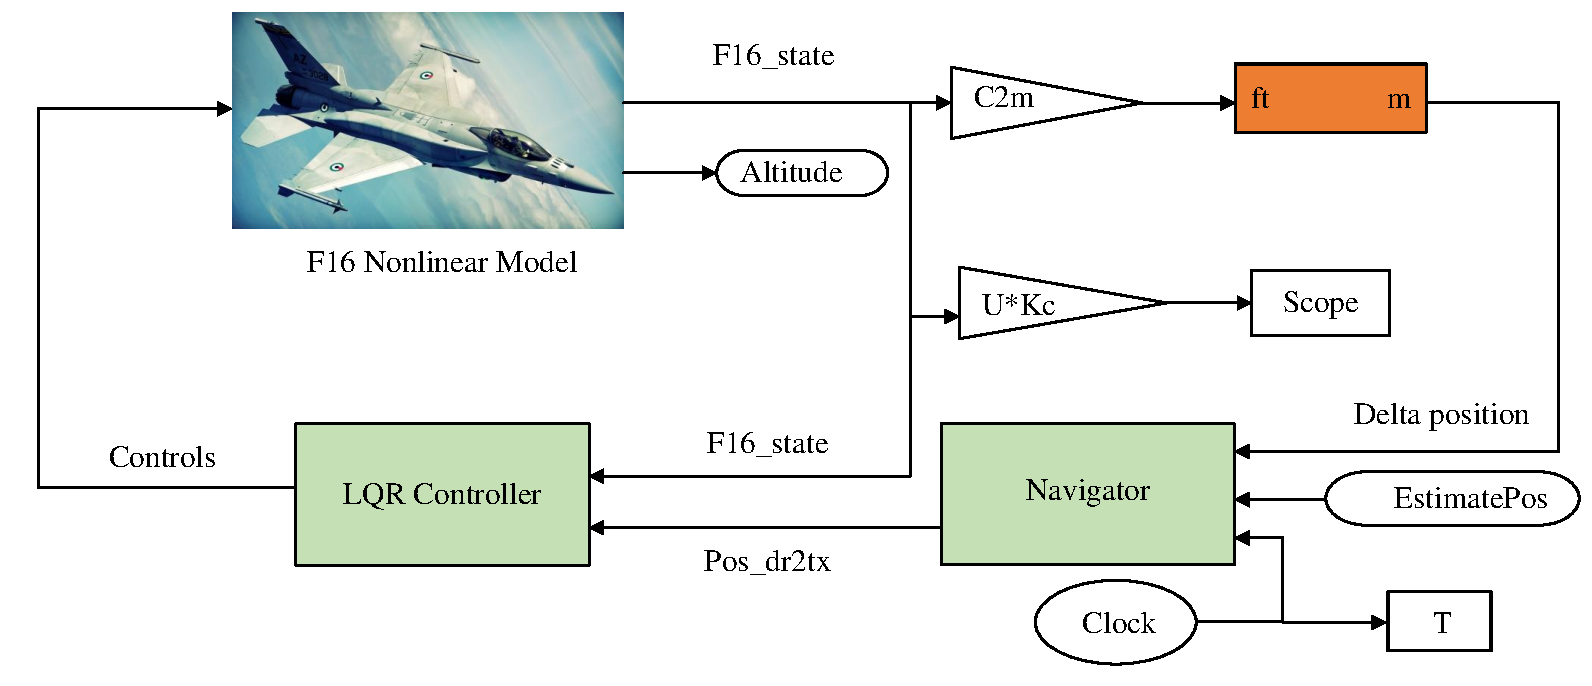
\includegraphics[width=0.9\textwidth]{Figures/Figs_Ch5/Fig15.pdf}
	\caption{The dataflow of Objective 1.}\label{FIG_15}
\end{figure}

\subsection{Implement of Objective 2}\label{sec5.3.2}
Compared to  Objective 1, the LQR controller is replaced with manual control via a joystick to complete the docking process. The pilot uses information of the receiver's states and relative position from the tanker to control the joystick for docking in Figure \ref{FIG_16}.

\begin{figure}[th]
	\centering
	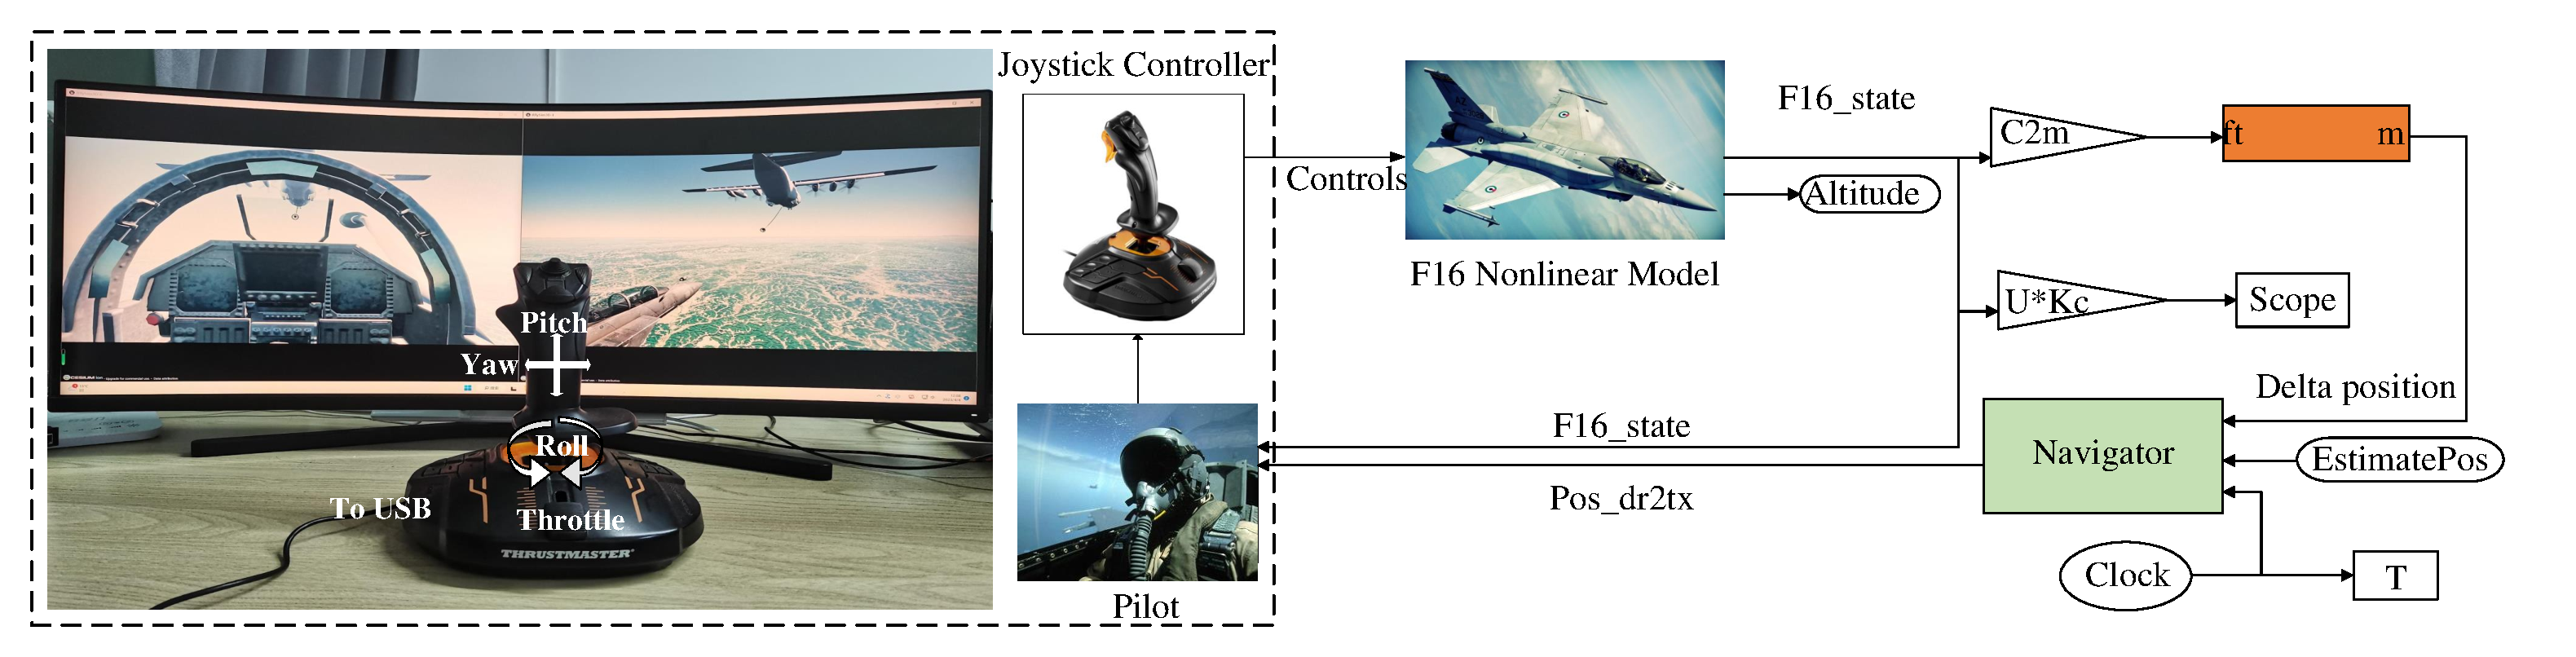
\includegraphics[width=1\textwidth]{Figures/Figs_Ch5/Fig16.pdf}
	\caption{The dataflow of Objective 2.}\label{FIG_16}
\end{figure}

To be specific, the joystick is connected to the simulation computer via USB to establish a connection with the simulation platform. As shown in Figure \ref{FIG_16}, the forward and backward movement of the joystick corresponds to the pitch of the receiver, while the left and right movement corresponds to the yaw. Clockwise and counterclockwise rotation corresponds to the roll, and the bottom slider corresponds to the throttle. 

\subsection{Results and analysis}\label{sec5.4}
Objective 2 is the same as Objective 1, hence the results and analysis of Objective 1 are presented in this part. Based on the settings and designs before, several successful docking attempts are accomplished. Figure \ref{FIG_17} shows the moment of both failed and successful docking. And the whole process of the AAR in the simulation of different phases is shown in Figure \ref{FIG_18} that is corresponds to Figure \ref{FIG_13}. The analysis will be illustrated from stability and motion mode, wind turbulence, hose tension monitoring, and docking accuracy respectively.
\begin{figure}[th]
	\centering
	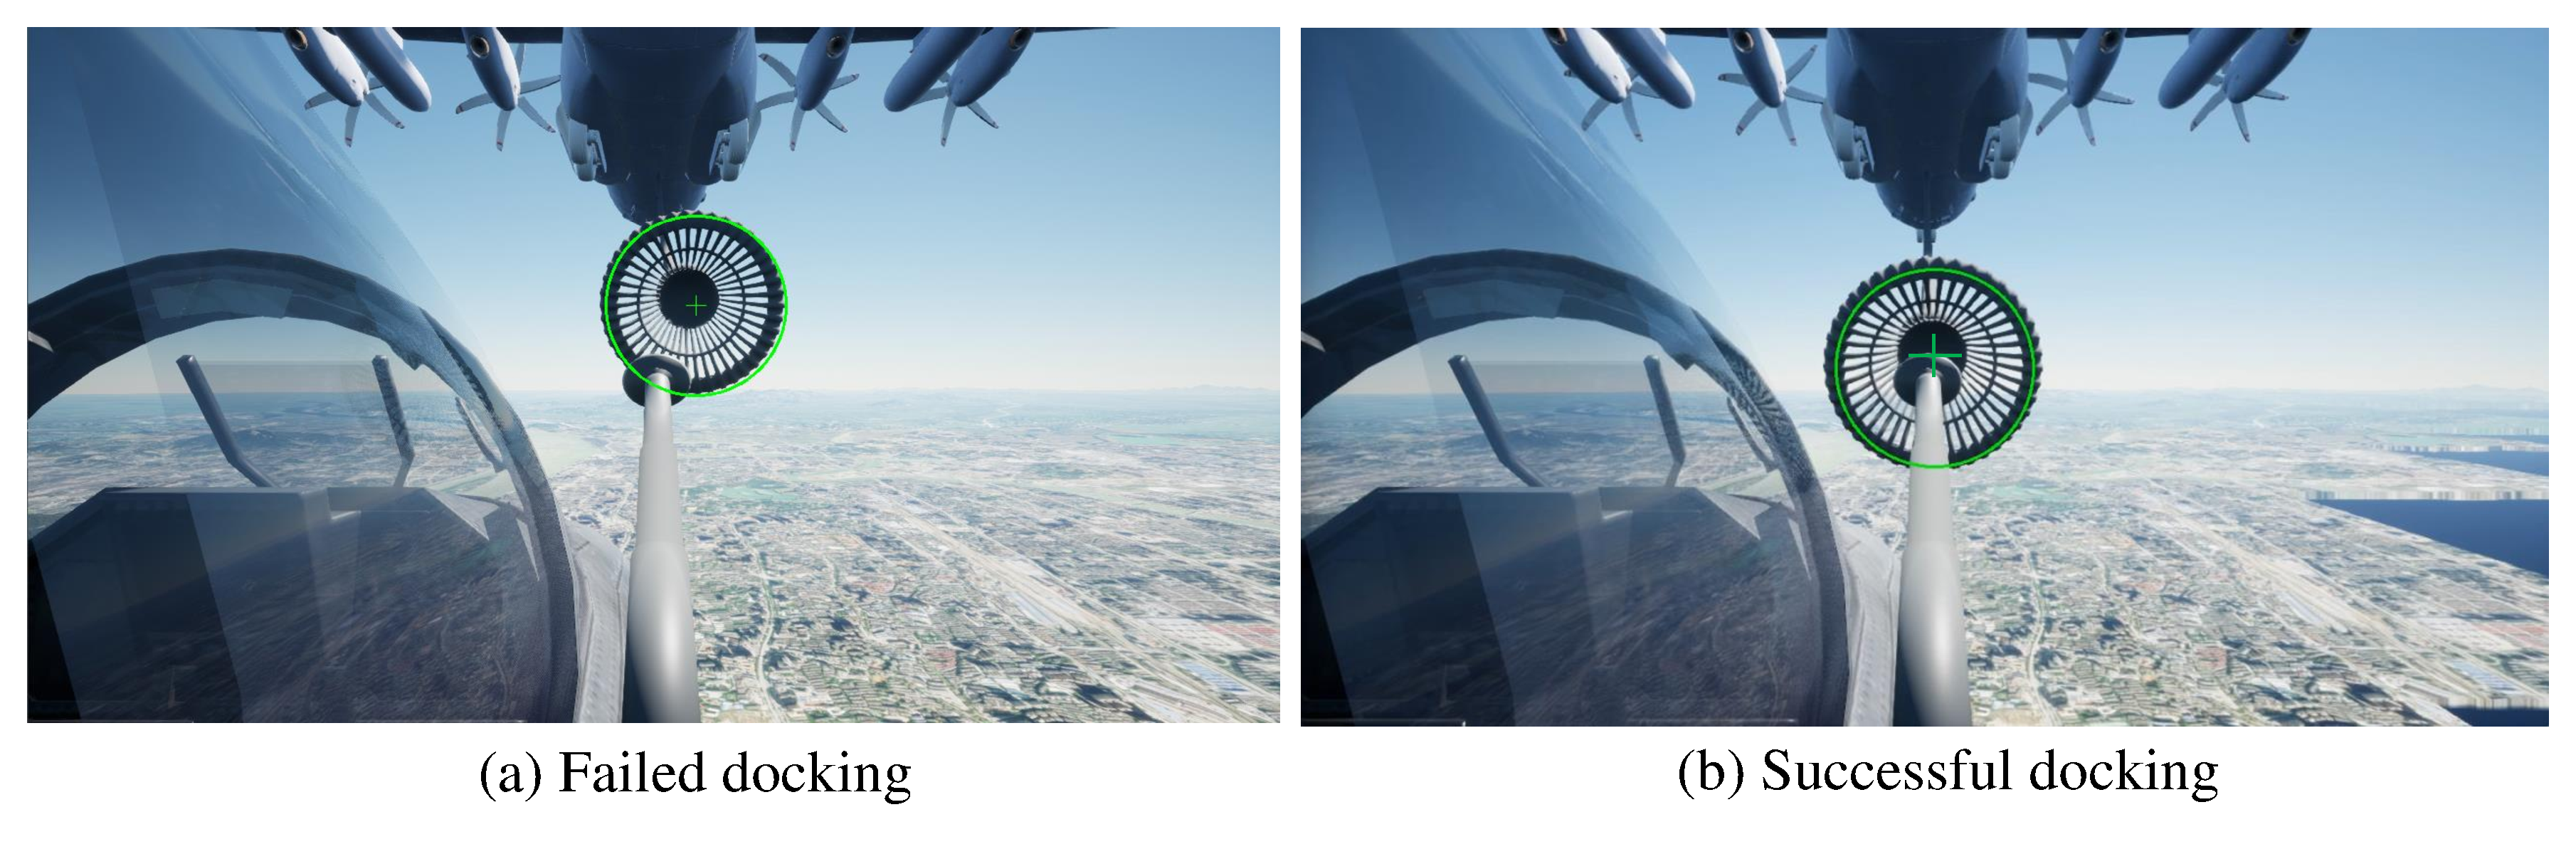
\includegraphics[width=0.9\textwidth]{Figures/Figs_Ch5/Fig17.pdf}
	\caption{The docking moment.}\label{FIG_17}
\end{figure}
\subsection{ Stability and motion mode}\label{sec5.4.1}
The linearized system can be divided into lateral and longitudinal systems to design controllers which should take the stability and the flight mode of the receiver into consideration. To avoid repeating the analysis of the system, the section takes the longitudinal system as an example. When giving the receiver a pulse of the elevator deflection, the responses of each state variable of the longitudinal motion are shown in Figure \ref{FIG_19}. The variation of airspeed and attack angle are selected to illustrate the different modes of the receiver. The variation of the speed corresponds to the phugoid mode which is determined by a pair of small conjugate complex roots. It has the characteristics of a long oscillation period and slow decay. The variation of the attack angle corresponds to the short period mode which is determined by a pair of roots with larger values. The oscillation period is shorter, decay is faster.

\begin{figure}[htp]
	\centering
	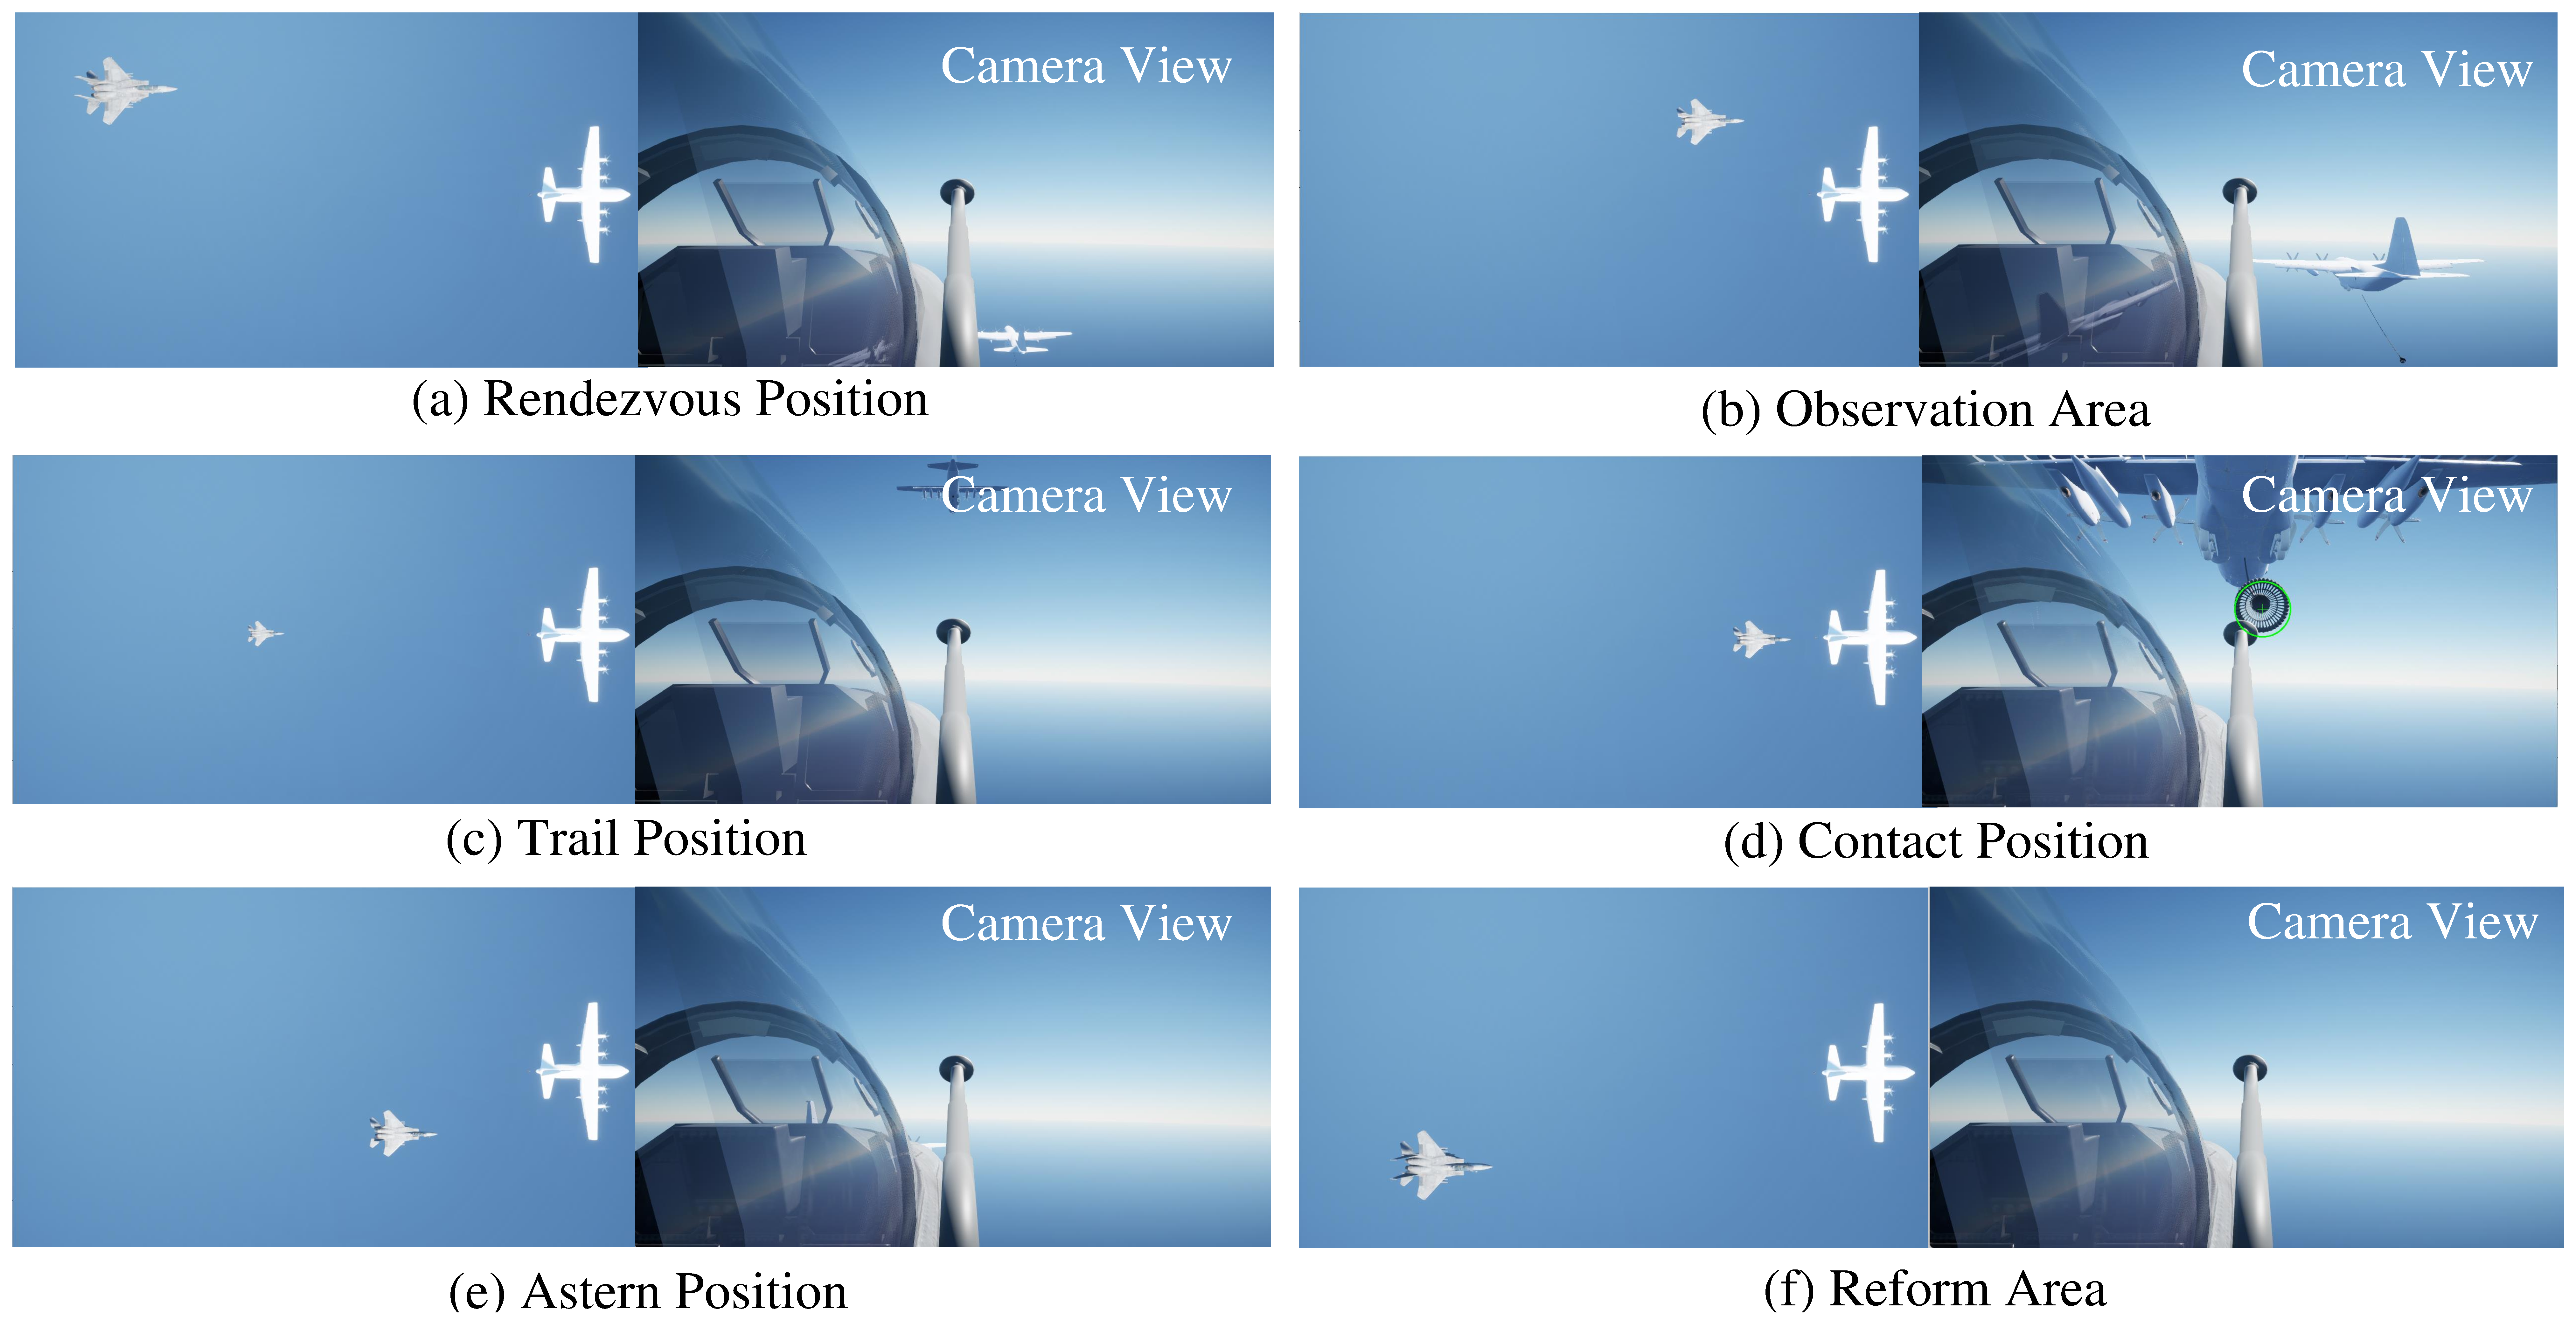
\includegraphics[width=1\textwidth]{Figures/Figs_Ch5/Fig18.pdf}
	\caption{God view(left) and onboard camera view(right).}\label{FIG_18}
\end{figure}

\begin{figure}[htpb]
	\centering
	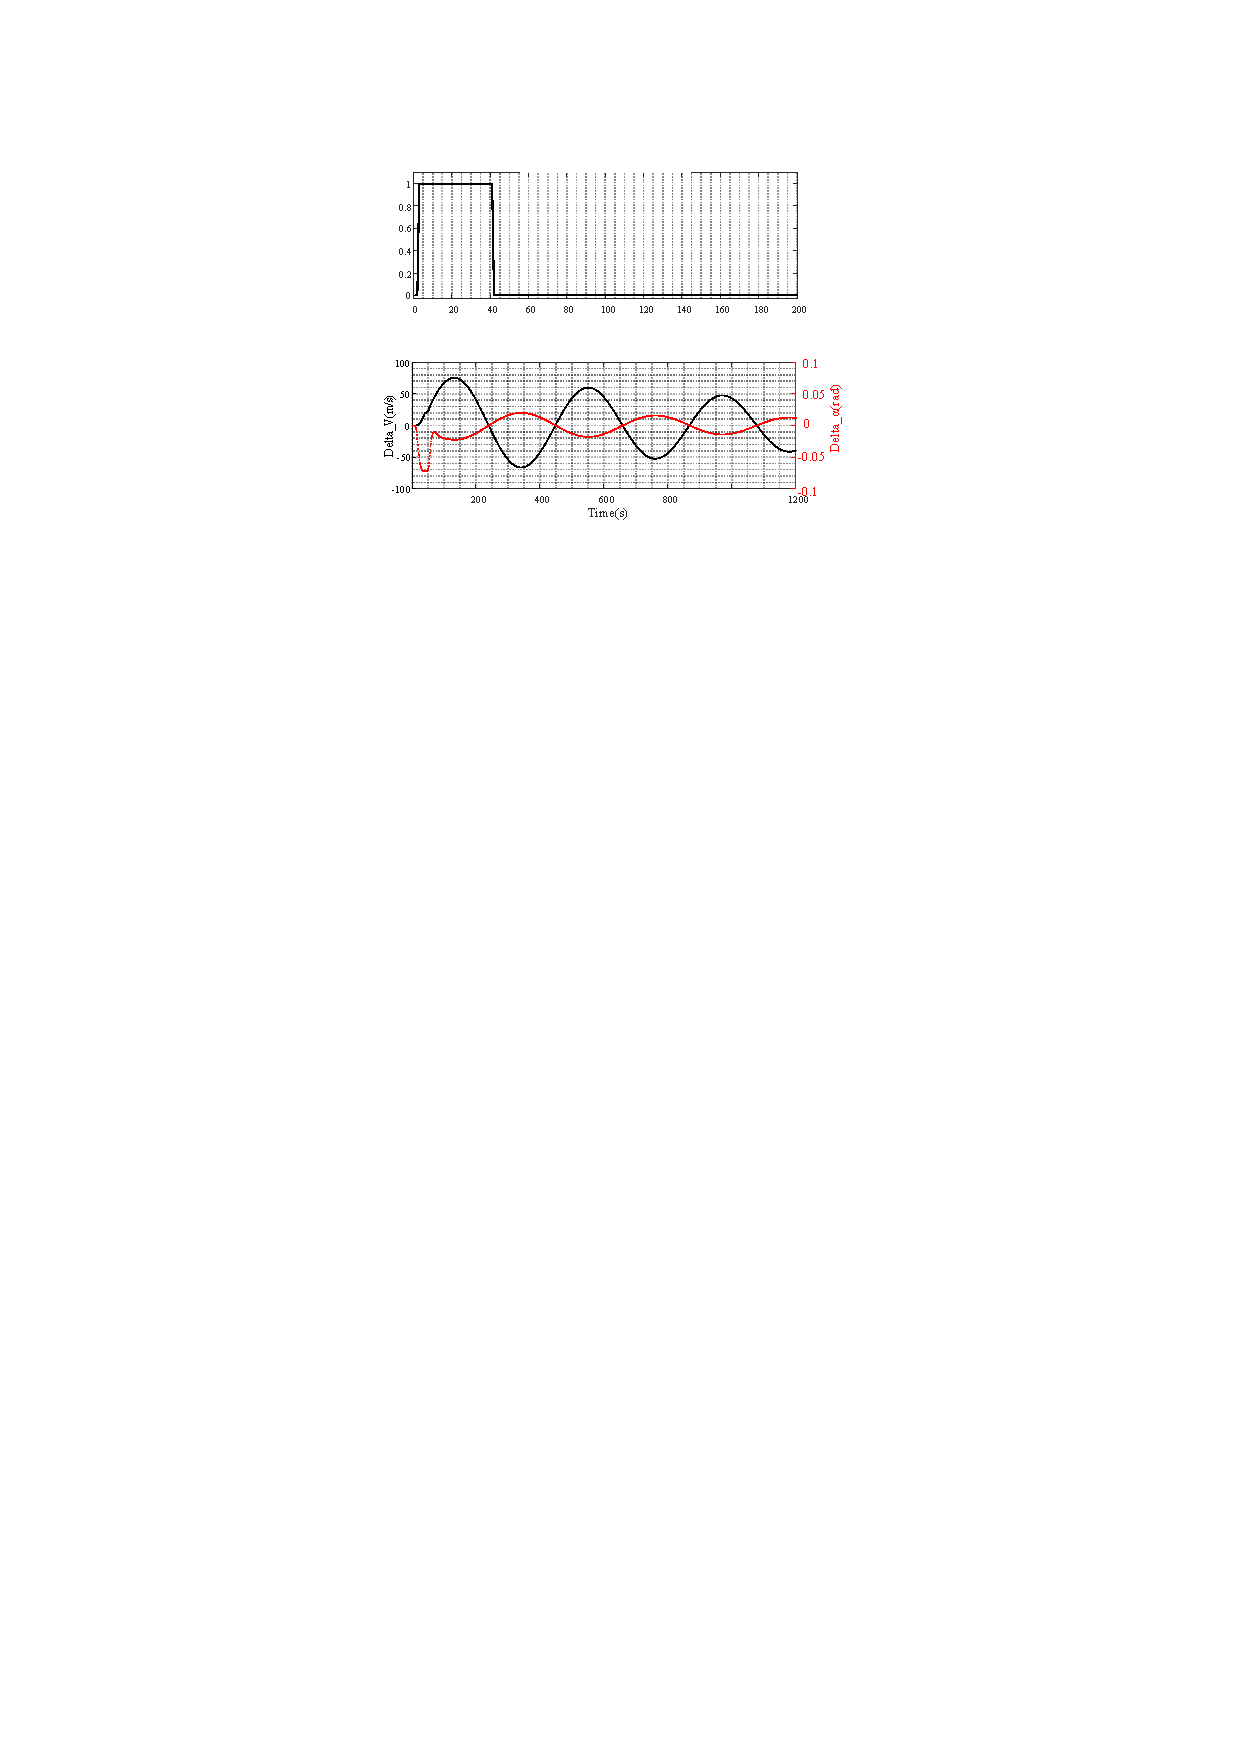
\includegraphics[width=0.7\textwidth]{Figures/Figs_Ch5/Fig19.pdf}
	\caption{Response of elevator pulse.}\label{FIG_19}
\end{figure}

Figure \ref{FIG_19} shows the system cannot keep stable when input has changed, hence the LQR controller is introduced to improve the system's performance. The results with and without the LQR controller are compared in Figure \ref{FIG_20}. On the condition of adopting the LQR controller, the aircraft climbed to a certain position swiftly and become stabilized, which demonstrates great maneuverability and stability.

\subsection{ Wind turbulence and hose tension monitoring}\label{sec5.4.2}
Then, the model is applied to the platform to simulate a docking process. During the process, the turbulence and the hose tension can be obtained for analysis. As mentioned above, the wind turbulences will disturb the drogue's movement and the HDU can suppress HWP. The turbulences containing bow wave effect, wake turbulence and natural wind, and hose tension are shown in Figure \ref{FIG_21}(a)-(c), which show the variety of the force caused by total turbulence in 7 successful docking processes. The curve shows the significant influence of the bow wave effect since they share a similar trend which just differs in offsets. When the probe approaches the drogue, the force in total turbulence increases tremendously. In addition, the HDU model has been applied to control the hose-drogue model which prevents excessive contact and the HWP effect. The real-time monitoring data of the hose tension is shown in Figure \ref{FIG_21} (d). The original tension of the hose is set to 1610 N and every trough represents the successful docking during the simulation. 



\begin{figure}[hp]
	\centering
	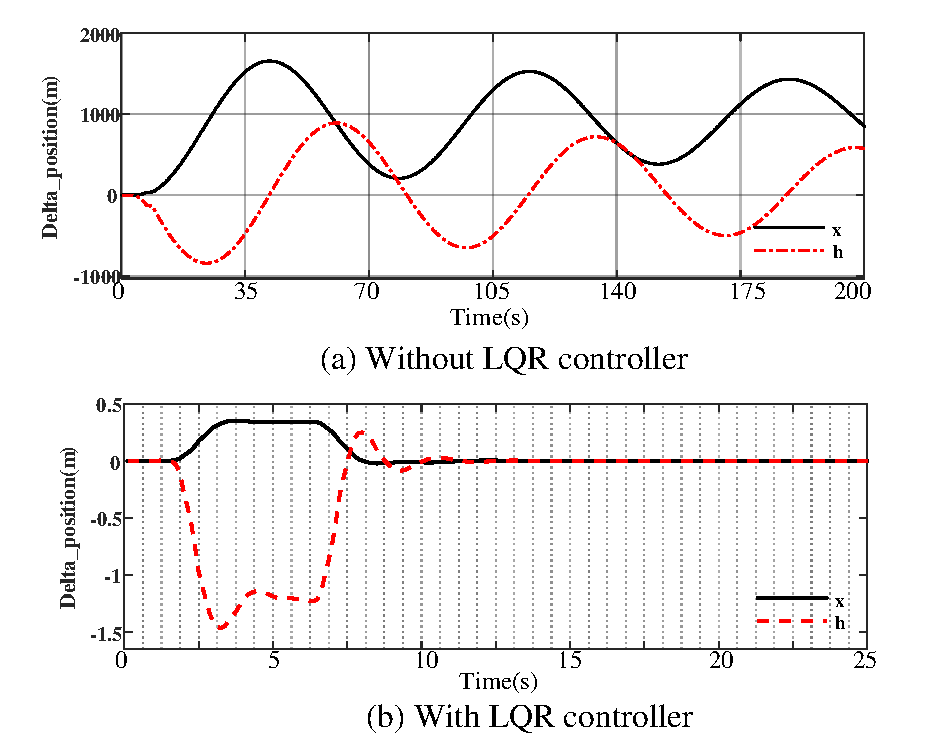
\includegraphics[width=0.7\textwidth]{Figures/Figs_Ch5/Fig20.pdf}
	\caption{The effect of the LQR controller.}\label{FIG_20}
\end{figure}

The HDU controller exerts an influence on the adjustment of the hose tension to prevent excessive contact in a complete docking process. In Figure \ref{FIG_22}(a), the receiver starts to approach the tanker from 30s to $ t_1 $and the probe gets in contact with the drogue at $ t_1 $. The hose remains the same length during this period. Then the probe drives the drogue to fly forward between  $ t_1 $ and $  t_2 $. The slack degree of the hose varies for the contact, which will lead to a change of the tension. At the same time, the HDU controller keeps the slack degree of the hose at a minimal value to accommodate this period. The probe and the drogue fly forward with a relatively static mode from $  t_2 $ to $  t_3 $ . The hose slack rate degree returns to 0 quickly and almost no changes after 38s. The probe breaks away from the drogue at $  t_3 $ which means a successful docking has been finished. The delta offset in the y axis and z axis are kept in a small region to ensure the accuracy and stationarity of the docking. In Figure \ref{FIG_22}(b), the distributions of the three parameters are all very close to zero, and their fluctuations are very small. Some of the outliers correspond to the peaks and valleys in Figure \ref{FIG_22} (a). The reason for these outliers is that the position of the drogue is deviated due to the wind disturbance during the flight process. Hence the HDU controller can effectively avoid HWP and guarantee the stationarity and safety of the refueling system.

\begin{figure}[htpb]
	\centering
	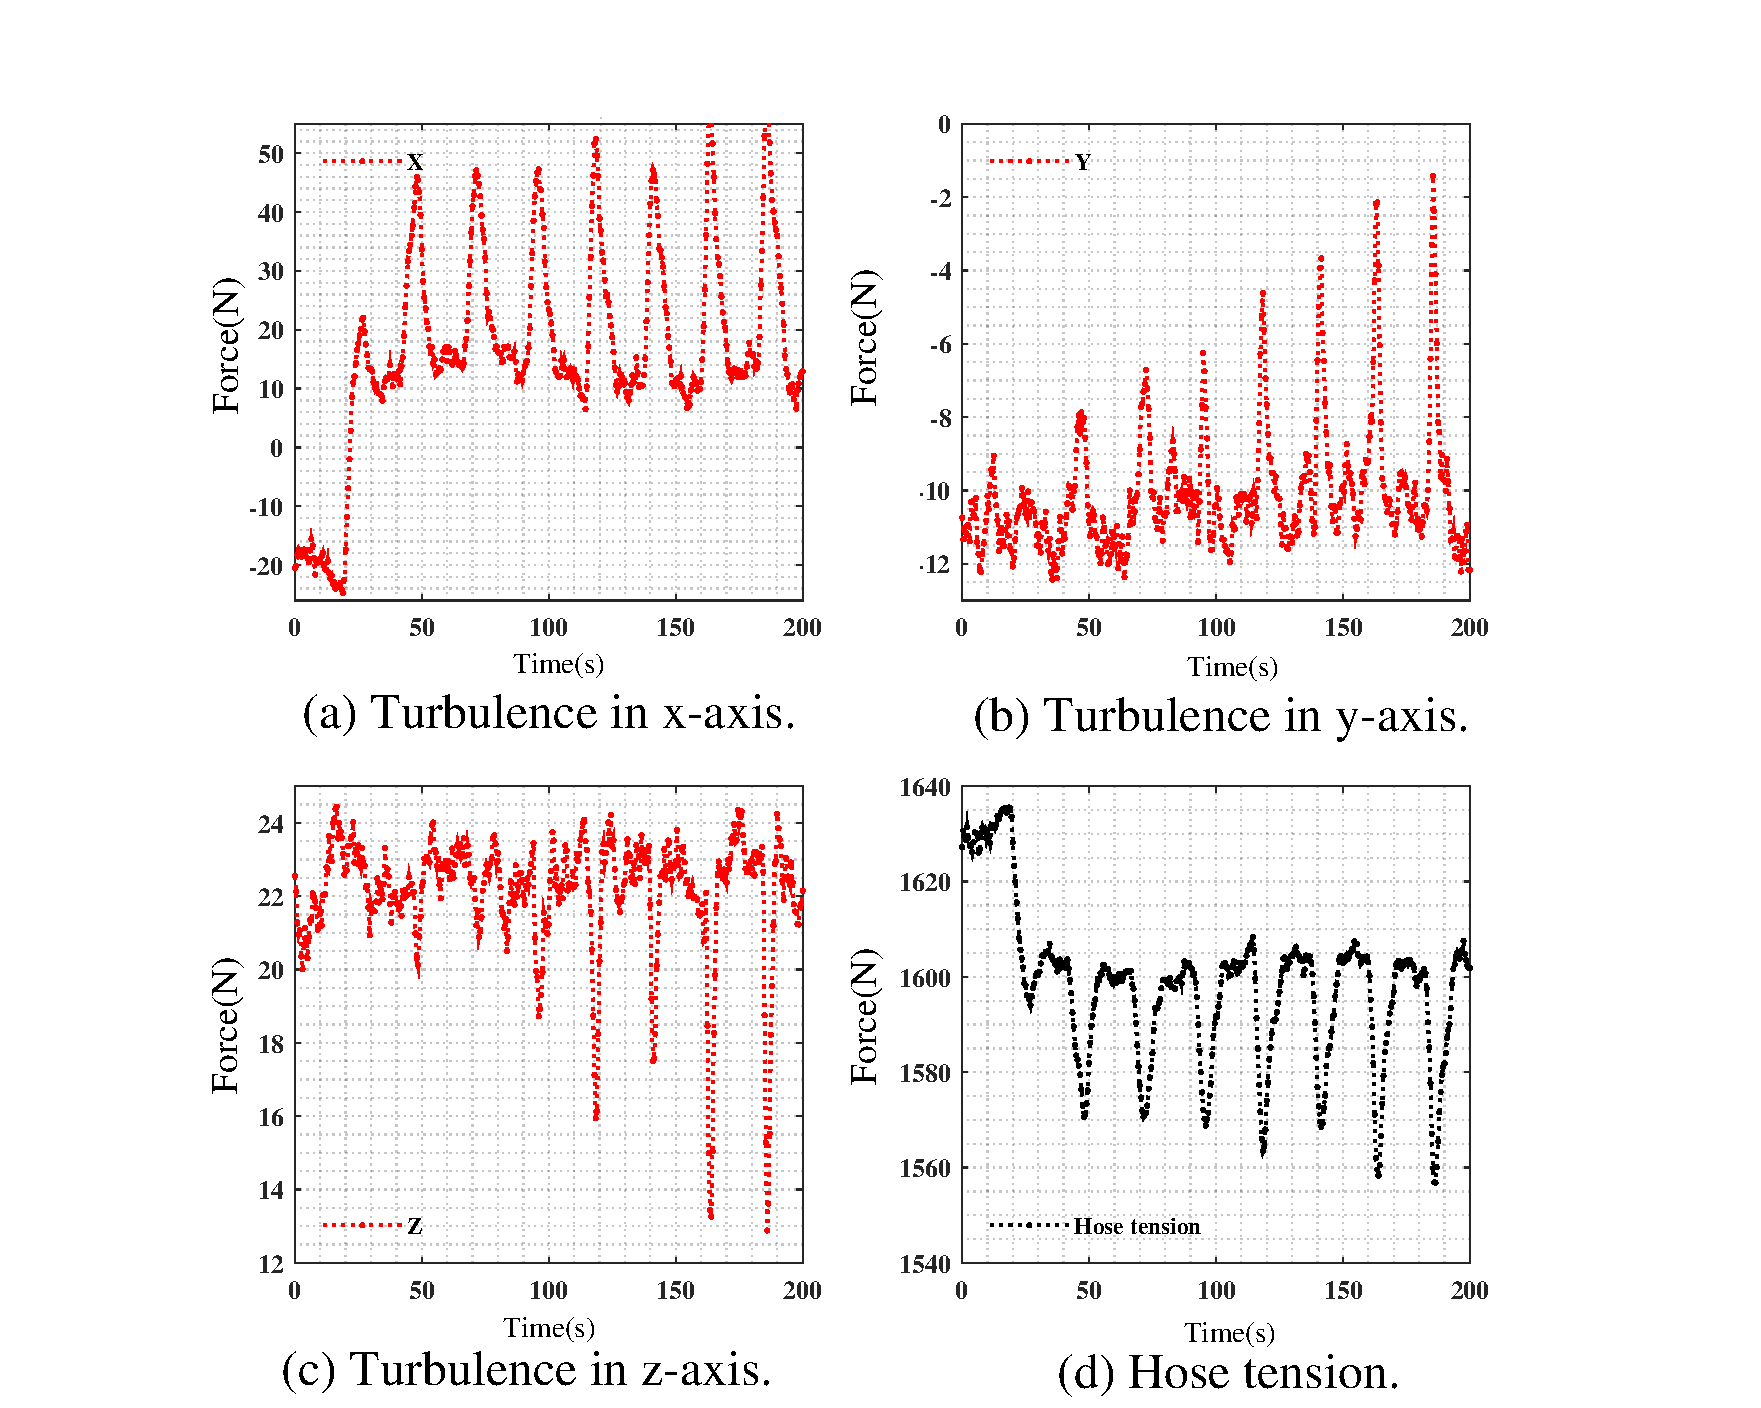
\includegraphics[width=0.6\textwidth]{Figures/Figs_Ch5/Fig21.pdf}
	\caption{ Hose tension and total turbulence.}\label{FIG_21}
\end{figure}

\begin{figure}[h]
	\centering
	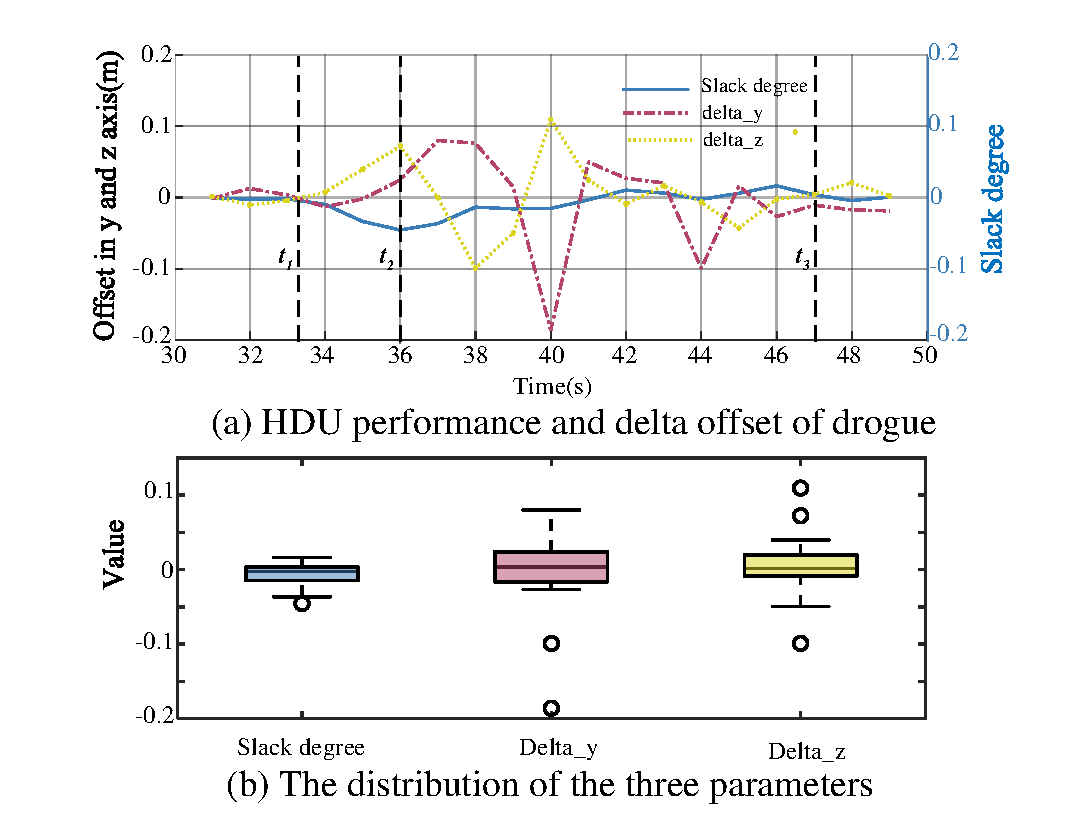
\includegraphics[width=0.5\textwidth]{Figures/Figs_Ch5/Fig22.pdf}
	\caption{HDU controller performance.}\label{FIG_22}
\end{figure}

\subsection{ Docking accuracy}\label{sec5.4.3}
A successful docking has been shown in Figure \ref{FIG_23} The refueling phase matches the time from the 40$ ^{\rm{th}} $ second to the 50$ ^{\rm{th}} $ second. The error is ${\rm{e}}_{{{\rm{dr}}}}^{{\rm{pr}}} = {\left[ {0.023  - 0.05 0.069} \right]^{\rm{T}}} $   which satisfies the requirement  
$\Delta R = 0.0884 < {R_{\rm{C}}}$   . After performing the refueling task, the receiver maneuvers back to the initial position which means the accomplishment of the third and the fourth phase.

\begin{figure}[ht]
	\centering
	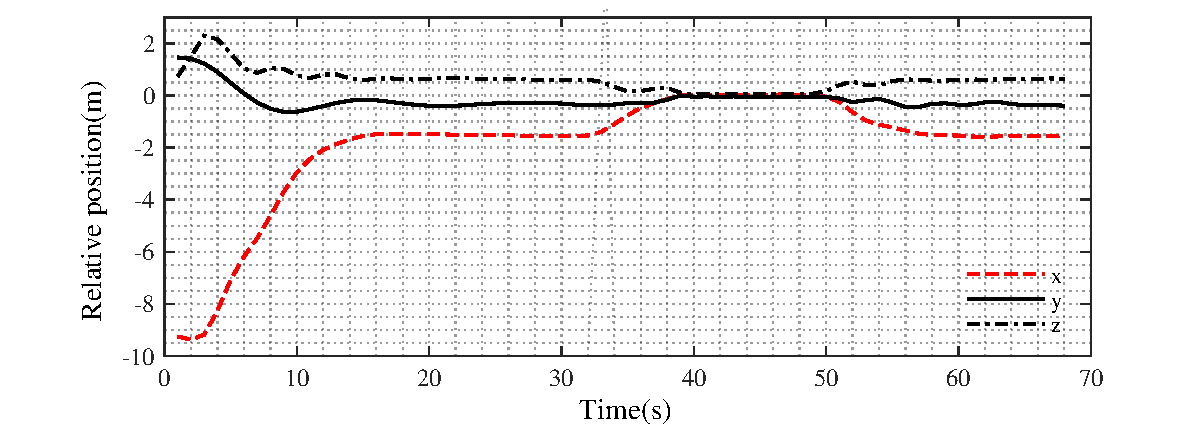
\includegraphics[width=0.7\textwidth]{Figures/Figs_Ch5/Fig23.pdf}
	\caption{Successful docking process.}\label{FIG_23}
\end{figure}

\subsection{Source code and video}\label{sec5.5}
The MATLAB$ ^{\rm{TM}} $/Simulink$^\circledR$ source code of AARSim is published on GitHub:

\begin{center}
	https://github.com/kelearnliu/AARSim
\end{center}

A video has been published to demonstrate AARSim, which includes an introduction to the platform, simulation procedures, and two demos as illustrated in Section \ref{sec5.1}:

\begin{center}
	https://v.youku.com/v\_\ show/id\_\ XNTk2NTAzMTMzMg==.html 
\end{center}

\section{Chapter Summary}
\label{sec6}
This paper proposes a simulation platform for AAR that is of great help to scientific research and education. AARSim is developed based on MATLAB$ ^{\rm{TM}} $/Simulink$^\circledR$ which contains aircraft models, refueling equipment model (with HDU model), and air disturbance models (incorporated with wind turbulence, wind gust, and wake turbulence of tanker) and bow wave effect. More importantly, a 3D rendering engine is used to create high-fidelity scenarios and visualize the entire phases based on comprehensively modeling the process of AAR. The information relationship among various models and the interfaces provided in each subsystem which can be modified according to the actual situation is illustrated in detail. The platform not only supports the more deep-going and more refined modeling of every model in the AAR process in modular form but improves the development efficiency of concerned algorithms tremendously with low cost. Meanwhile, the co-simulation of Python and MATLAB$ ^{\rm{TM}} $/Simulink$^\circledR$ extends the availability, which can utilize abundant methods in perception and control.

